\documentclass[journal=jprobs,manuscript=article]{achemso}
\usepackage[utf8]{inputenc}
\usepackage{amsmath}
\usepackage{bm}
\usepackage[dvipsnames]{xcolor}
\usepackage{hyperref}
\usepackage{fancyhdr}
\usepackage{graphicx}
\pagestyle{fancy}
\fancyhf{}
\cfoot{S-\thepage}

%\usepackage{changepage}   % For adjusting image width
%\usepackage{xr}

\fancypagestyle{firststyle}
{
   \fancyhead[R]{}
   \fancyhead[L]{}
   \fancyfoot[C]{}
}

\fancyfoot[C]{S-\thepage}
\fancyhead[R]{\textit{\small{Mouse primary T cell phosphoyrosine proteomics enabled by BOOST}}}
%\fancyhead[L]{\small{Chua \& Callahan \textit{et al.}}}
\fancyhead[L]{\small{Chua \& Callahan \textit{et al.}}}
\renewcommand{\figurename}{Supporting Figure}   % Renaming the Figure float name to "Supplementary Figure"
\renewcommand{\tablename}{Supporting Table}     % Renaming the Table float name to "Supplementary Table"
\newcommand\XOR{\mathbin{\char`\^}}

%%%%%%%%%%%%%%%%%%%%%%%%%%%%%%%%%%%%%%%%%%%%%%%%%%%%%%%%%%%%%%%%%%%%%%%%%%%%
% Originally, this was used to create a \beginsupplement command that would
% renumber and rename the figures and tables like above, however I removed
% this when I made the supplements their own document.
%\newcommand{\beginsupplement}{%
%            \setcounter{table}{0}
%            \renewcommand{\thetable}{Supplementary Table \arabic{table}}%
%            \setcounter{figure}{0}
%            \renewcommand{\thefigure}{\arabic{figure}}%
%     }
%%%%%%%%%%%%%%%%%%%%%%%%%%%%%%%%%%%%%%%%%%%%%%%%%%%%%%%%%%%%%%%%%%%%%%%%%%%%
\title{Supporting Information:  \\Mouse primary T cell phosphoyrosine proteomics enabled by BOOST}

\author{Xien Yu Chua$^{1,\P}$, Kenneth P. Callahan$^{2,\P}$, Alijah A. Griffith$^{2}$, Tobias Hildebrandt$^{1}$, Guoping Fu$^{3}$, Mengzhou Hu$^{1}$, Renren Wen$^{3}$, Arthur R. Salomon$^{2,*}$
\\
\singlespacing
\textit{\small{$1$ Department of Molecular Pharmacology, Physiology \& Biotechnology, Brown University, Providence, RI, 02912}}
\\
\textit{\small{$2$ Department of Molecular Biology, Cell Biology \& Biochemistry, Brown University, Providence, RI, 02912}}
\\
\textit{\small{$3$ Blood Research Institute, Blood Center of Wisconsin, Milwaukee, WI, 53226}}
\\
\textit{\small{$\P$ Contributed equally to this work}}
\\
\textit{\small{$*$} Corresponding Author}\tiny}
\email{art@drsalomon.com}
%\\
%\textit{\small{$\P$ Contributed equally to this work}}\tiny}
%
%
% In our previous manuscript submission using LaTeX (https://doi.org/10.1021/acs.jproteome.1c00735),
% The editors of JPR wanted the author affiliations to be numbered, rather than
% the symbols automatically provided by the achemso package. 
%
% To get back to the original code, just comment out the lines above and uncomment the
% lines below.

%\author{Xien Yu Chua}
%\altaffiliation{Contributed equally to this work}
%\affiliation{Department of Molecular Pharmacology, Physiology \& Biotechnology, Brown University, Providence, RI, 02912}
%\author{Kenneth P. Callahan}
%\altaffiliation{Contributed equally to this work}
%\author{Alijah A. Griffith}
%\affiliation{Department of Molecular Biology, Cell Biology \& Biochemistry, Brown University, Providence, RI, 02912}
%\author{Tobias Hildebrandt}
%\affiliation{Department of Molecular Pharmacology, Physiology \& Biotechnology, Brown University, Providence, RI, 02912}
%\author{Guoping Fu}
%\affiliation{Blood Research Institute, Blood Center of Wisconsin, Milwaukee, WI, 53226}
%\author{Mengzhou Hu} 
%\affiliation{Department of Molecular Pharmacology, Physiology \& Biotechnology, Brown University, Providence, RI, 02912}
%\author{Arthur R. Salomon}
%\email{art@drsalomon.com}
%\affiliation[Brown University]{Department of Molecular Biology, Cell Biology \& Biochemistry, Brown University}

%\date{September 2021}

\begin{document}
\pagenumbering{gobble}
\thispagestyle{firststyle}
\newpage
\begin{center}
\textbf{\underline{\large{Table Of Contents}}}
\end{center}

%\begin{table}[h!]
%    \begin{tabular}{ll}
%        \textbf{\hyperref[silaclabelingtable]{Supplementary Table} \ref{silaclabelingtable}:} & (.XLSX) Complete list of peptides identified after heavy   \\
%         & isotope labeling of Raji B cells and their labeling status. \\
%
 %       \textbf{\hyperref[ssh2totaltable]{Supplementary Table} \ref{ssh2totaltable}:} & (.XLSX) All peptides identified from sSH2 pTyr enrichment  \\
 %        & after coculture of CD19-CAR T cells and Raji B cells. \\
%
%        \textbf{\hyperref[tio2totaltable]{Supplementary Table} \ref{tio2totaltable}:} & (.XLSX) All peptides identified from TiO$_2$ phosphopeptide \\
%        & enrichment after coculture of CD19-CAR T cells and Raji B \\
%        & cells. \\
%    \end{tabular}
%\end{table}
\pagenumbering{arabic}
\setcounter{page}{1}

\begin{table}[h!]
    \begin{tabular}{ll}

        \textbf{\hyperref[boost_gained_peps]{Supporting Table} \ref{boost_gained_peps}:} & (.XLSX) All unique peptides observed in the BOOST \\
                                                                                                                                                  & experiment without $\Phi$SDM \\

	\textbf{\hyperref[nosdm_overlap_peps]{Supporting Table} \ref{nosdm_overlap_peps}:} & (.XLSX) All unique peptides observed in the BOOST \\
                                                                                                                                                         & and $1.0$ mg Control experiments without $\Phi$SDM \\
	\textbf{\hyperref[control_only_peps]{Supporting Table} \ref{control_only_peps}:} & (.XLSX) All unique peptides observed in the $1.0$ mg \\
                                                                                                                                                  & Control experiment without $\Phi$SDM \\

	\textbf{\hyperref[boostsdm_gained_peps]{Supporting Table} \ref{boostsdm_gained_peps}:} & (.XLSX) All unique peptides observed in the BOOST \\
                                                                                                                                                  & experiment with $\Phi$SDM \\

	\textbf{\hyperref[sdm_overlap_peps]{Supporting Table} \ref{sdm_overlap_peps}:} & (.XLSX) All unique peptides observed in the BOOST \\
                                                                                                                                                         & and $1.0$ mg Control experiments with $\Phi$SDM \\

	\textbf{\hyperref[controlsdm_only_peps]{Supporting Table} \ref{controlsdm_only_peps}:} & (.XLSX) All unique peptides observed in the $1.0$ mg\\
                                                                                                                                                  & Control experiment with $\Phi$SDM \\

	\textbf{Supporting Folder 1} & (.ZIP) All tables output from MaxQuant \\

	\textbf{Supporting Folder 2} & (.ZIP) All Python3 code used for data analysis \\

        \textbf{\hyperref[locprob]{Supporting Figure} \ref{locprob}:} & Histogram of all PSMs containing a phosphory- \\
                                                                                                                & lated amino acid in all conditions binned by \\
                                                                                                                & localization probability \\

       \textbf{\hyperref[nancounts]{Supporting Figure} \ref{nancounts}:} & Missing value bar charts for each experiment \\

        \textbf{\hyperref[intensity_plots]{Supporting Figure} \ref{intensity_plots}:} & $\log_{10}$ transformed reporter intensity box-and- \\
                                                                                                                                   & whisker plots \\

	\textbf{\hyperref[mg1_repmean]{Supporting Figure} \ref{mg1_repmean}:} & Comparison of replicate intensities to the\\
													    & mean of each pTyr peptide PSM in the $1.0$ mg\\
													    & condition. \\

	\textbf{\hyperref[mg03_repmean]{Supporting Figure} \ref{mg03_repmean}:} & Comparison of replicate intensities to the\\
													    & mean of each pTyr peptide PSM in the $0.3$ mg\\
													    & condition. \\

	\textbf{\hyperref[mg01_repmean]{Supporting Figure} \ref{mg01_repmean}:} & Comparison of replicate intensities to the\\
													    & mean of each pTyr peptide PSM in the $0.1$ mg\\
													    & condition. \\
        
        \textbf{\hyperref[boost_replicate_reprod]{Supporting Figure} \ref{boost_replicate_reprod}:} & Pairwise replicate comparisons of unique PSMs  \\
                                                                                                                                                                    &  identified in BOOST when $\Phi$SDM is disabled \\

        \textbf{\hyperref[boostsdm_replicate_reprod]{Supporting Figure} \ref{boostsdm_replicate_reprod}:} & Pairwise replicate comparisons of unique PSMs  \\
                                                                                                                                                                    &  identified in BOOSTwhen $\Phi$SDM is enabled \\

        \textbf{\hyperref[control_replicate_reprod]{Supporting Figure} \ref{control_replicate_reprod}:} & Pairwise replicate comparisons of unique PSMs  \\
                                                                                                                                                                    &  identified in$1.0$ mg Control when $\Phi$SDM\\
                                                                                                                                                                    &  is disabled \\

        \textbf{\hyperref[controlsdm_replicate_reprod]{Supporting Figure} \ref{controlsdm_replicate_reprod}:} & Pairwise replicate comparisons of unique peptides  \\
                                                                                                                                                                    &  identified in$1.0$ mg Control when $\Phi$SDM\\
                                                                                                                                                                    &  is enabled \\

    \end{tabular}
\end{table}

\clearpage

\begin{table}[h!]
    \begin{tabular}{ll}

        \textbf{\hyperref[boost_control_gained_qvolcanoes]{Supporting Figure} \ref{boost_control_gained_qvolcanoes}:} & Venn Diagram and Volcano Plots for BOOST  \\
                                                                                                                                                                                                       &  and $1.0$ mg Control when $\Phi$SDM is disabled \\
%                                                                                                                                                                                                       &  \\

        \textbf{\hyperref[boostsdm_controlsdm_gained_qvolcanoes]{Supporting Figure} \ref{boostsdm_controlsdm_gained_qvolcanoes}:} & Venn Diagram and Volcano Plots for BOOST  \\
                                                                                                                                                                                                       &  and $1.0$ mg Control when $\Phi$SDM is enabled \\

        \textbf{\hyperref[set_overlap_2]{Supporting Figure} \ref{set_overlap_2}:} & Venn Diagrams for BOOST conditions (with   \\
                                                                                                                                       & and without $\Phi$SDM) and $1.0$ mg Control (with \\
                                                                                                                                       & and without $\Phi$SDM)\\

        \textbf{\hyperref[boost_factor_cdfs]{Supporting Figure} \ref{boost_factor_cdfs}:} & Cumulative distributions of unique pTyr pept- \\
                                                                                                                                                    & ides from BOOST experiments (with and \\
                                                                                                                                       & without $\Phi$SDM)\\

	\textbf{\hyperref[mouse_jurkat_keggtcr]{Supporting Figure} \ref{mouse_jurkat_keggtcr}:} &  Overlap between Mouse-BOOST and \\
                                                                                                                                                               & Jurkat-BOOST experiments \\

    \end{tabular}
\end{table}

\clearpage



% Space for the Supplemental Tables

\begin{table}[h!]
	\caption{All unique peptide PSMs observed exclusively in the BOOST experiment with $\Phi$SDM disabled and reporter ions quantified in at least one experimental channel. Included are MaxQuant outputs such as the gene name(s), protein name(s), modified sequence, modified sequence with phosphorylation site localization probabilities, sequence windows, and corrected TMT reporter ion intensities, as well as calculations used in the manuscript (mean intensity values, standard deviations, CV percentages, $p$-values, $q$-values, BOOST factors) and \href{https://www.wikipathways.org/index.php/WikiPathways}{WikiPathways}\cite{martens2021wikipathways} Annotations for each unique peptide.
}\label{boost_gained_peps}
\end{table}

\begin{table}[h!]
	\caption{All unique peptide PSMs observed in both the BOOST experiment and the 1.0 mg Control experiment with $\Phi$SDM disabled and reporter ions quantified in at least one experimental channel.  Included are MaxQuant outputs such as the gene name(s), protein name(s), modified sequence, modified sequence with phosphorylation site localization probabilities, sequence windows, and corrected TMT reporter ion intensities, as well as calculations used in the manuscript (mean intensity values, standard deviations, CV percentages, $p$-values, $q$-values, BOOST factors) and \href{https://www.wikipathways.org/index.php/WikiPathways}{WikiPathways}\cite{martens2021wikipathways} Annotations for each unique peptide.
}\label{nosdm_overlap_peps}
\end{table}

\begin{table}[h!]
	\caption{All unique peptide PSMs observed exclusively in the 1.0 mg Control experiment with $\Phi$SDM disabled and reporter ions quantified in at least one experimental channel.  Included are MaxQuant outputs such as the gene name(s), protein name(s), modified sequence, modified sequence with phosphorylation site localization probabilities, sequence windows, and corrected TMT reporter ion intensities, as well as calculations used in the manuscript (mean intensity values, standard deviations, CV percentages, $p$-values, $q$-values) and \href{https://www.wikipathways.org/index.php/WikiPathways}{WikiPathways}\cite{martens2021wikipathways} Annotations for each unique peptide.
}\label{control_only_peps}
\end{table}

\begin{table}[h!]
	\caption{All unique peptide PSMs observed exclusively in the BOOST experiment with $\Phi$SDM enabled and reporter ions quantified in at least one experimental channel.  Included are MaxQuant outputs such as the gene name(s), protein name(s), modified sequence, modified sequence with phosphorylation site localization probabilities, sequence windows, and corrected TMT reporter ion intensities, as well as calculations used in the manuscript (mean intensity values, standard deviations, CV percentages, $p$-values, $q$-values, BOOST factors) and  \href{https://www.wikipathways.org/index.php/WikiPathways}{WikiPathways}\cite{martens2021wikipathways} Annotations for each unique peptide.
}\label{boostsdm_gained_peps}
\end{table}

\begin{table}[h!]
	\caption{All unique peptide PSMs observed in both the BOOST experiment and the 1.0 mg Control experiment with $\Phi$SDM enabled and reporter ions quantified in at least one experimental channel.  Included are MaxQuant outputs such as the gene name(s), protein name(s), modified sequence, modified sequence with phosphorylation site localization probabilities, sequence windows, and corrected TMT reporter ion intensities, as well as calculations used in the manuscript (mean intensity values, standard deviations, CV percentages, $p$-values, $q$-values, BOOST factors) and  \href{https://www.wikipathways.org/index.php/WikiPathways}{WikiPathways}\cite{martens2021wikipathways} Annotations for each unique peptide.
}\label{sdm_overlap_peps}
\end{table}

\begin{table}[h!]
	\caption{All unique peptide PSMs observed exclusively in the 1.0 mg Control experiment with $\Phi$SDM enabled and reporter ions quantified in at least one experimental channel.  Included are MaxQuant outputs such as the gene name(s), protein name(s), modified sequence, modified sequence with phosphorylation site localization probabilities, sequence windows, and corrected TMT reporter ion intensities, as well as PhosphoSitePlus$^{\text{\textregistered}}$ site annotations, calculations used in the manuscript (mean intensity values, standard deviations, CV percentages, $p$-values, $q$-values) and \href{https://www.wikipathways.org/index.php/WikiPathways}{WikiPathways}\cite{martens2021wikipathways} Annotations for each unique peptide.
}\label{controlsdm_only_peps}
\end{table}

% Change the numbering for the Supplemental Folders
% This is purely to create a numbered thing called "Supplementary Folder"
% that can be referenced.
\setcounter{table}{0}
\renewcommand{\tablename}{Supporting Folder}

\begin{table}[h!]
	\caption{All tables generated by MaxQuant as text files. These include ``summary.txt" (a summary of parameters, information, .raw files, and statistics used for peak detection), ``evidence.txt" (all information about unique peptides quantified from .raw files), ``peptides.txt" (information about the peptides identified from .raw files), ``modificationSpecificPeptides.txt" (information about posttranlational modifications to the peptides), ``Oxidation (M)Sites.txt" (information about oxidized peptides), ``Phospho (STY)Sites.txt" (information about phosphorylated peptides), ``proteinGroups.txt" (information about estimated protein abundance from the .raw files), ``allPeptides.txt" (all information for each unique peptide identified in each .raw file), ``msScans.txt" (information about the scans observed on the mass spectrometer), ``mzRange.txt", ``msmsScans.txt" (information about the MS/MS scans for each .raw file),  and ``msms.txt" (information about the MS/MS spectra for each peptide identified in each .raw file).}
\end{table}


\begin{table}
	\caption{All Python3 code used to analyze the MaxQuant output files and databases referenced. These include ``data\_analysis.py" (script used to generate plots), ``helpers/" (Python3 files used to assist in data analysis), ``database/" (all external databases used in analysis), and ``maxquant\_results" (the ``evidence.txt" and ``Phospho (STY)Sites.txt" files from Supporting Folder 2), as well as the output folders ``figures/" (all figures generated by data\_analysis.py) and ``curated\_results/" (all .txt output files from Python3 analysis, which are aggregated and formatted in Supporting Tables \ref{boost_gained_peps}-\ref{controlsdm_only_peps}).}
\end{table}

%\clearpage

%\begin{figure}[t!]
%\centering
%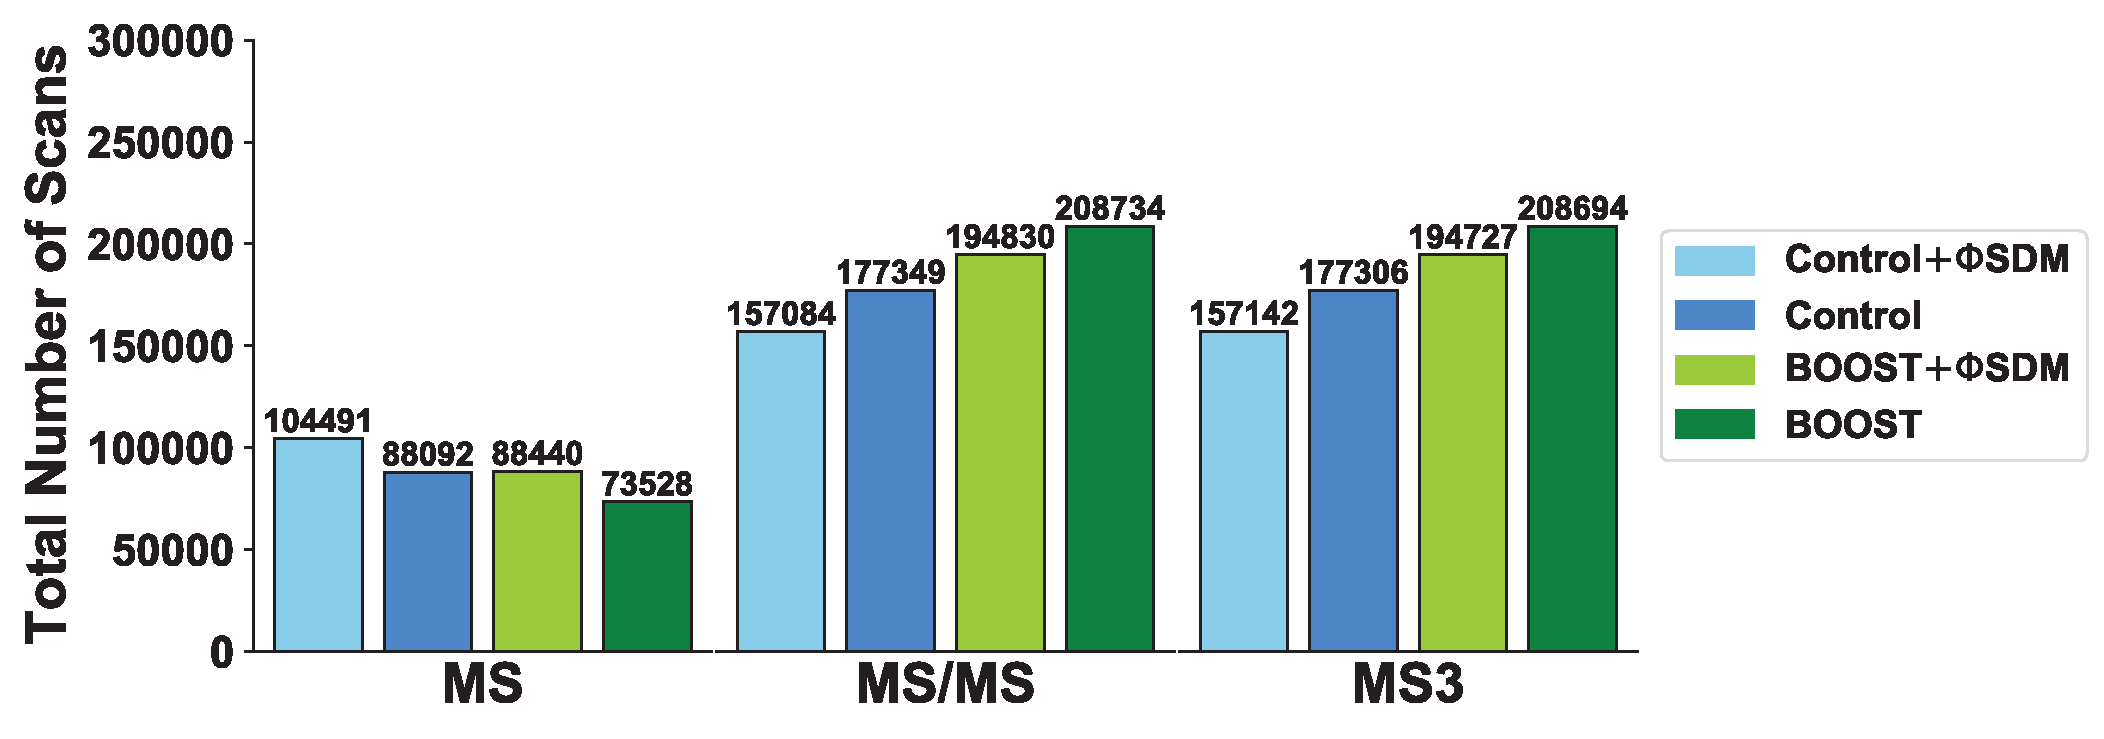
\includegraphics[width=175mm]{figures/supplements/scans.pdf}
%\caption{A bar chart showing the total number of MS, MS/MS and MS3 scans from each experiment. The numbers above each bar indicate the exact number of scans for that experiment. }\label{scans}
%\end{figure}

\clearpage

\begin{figure}[t!]
\centering
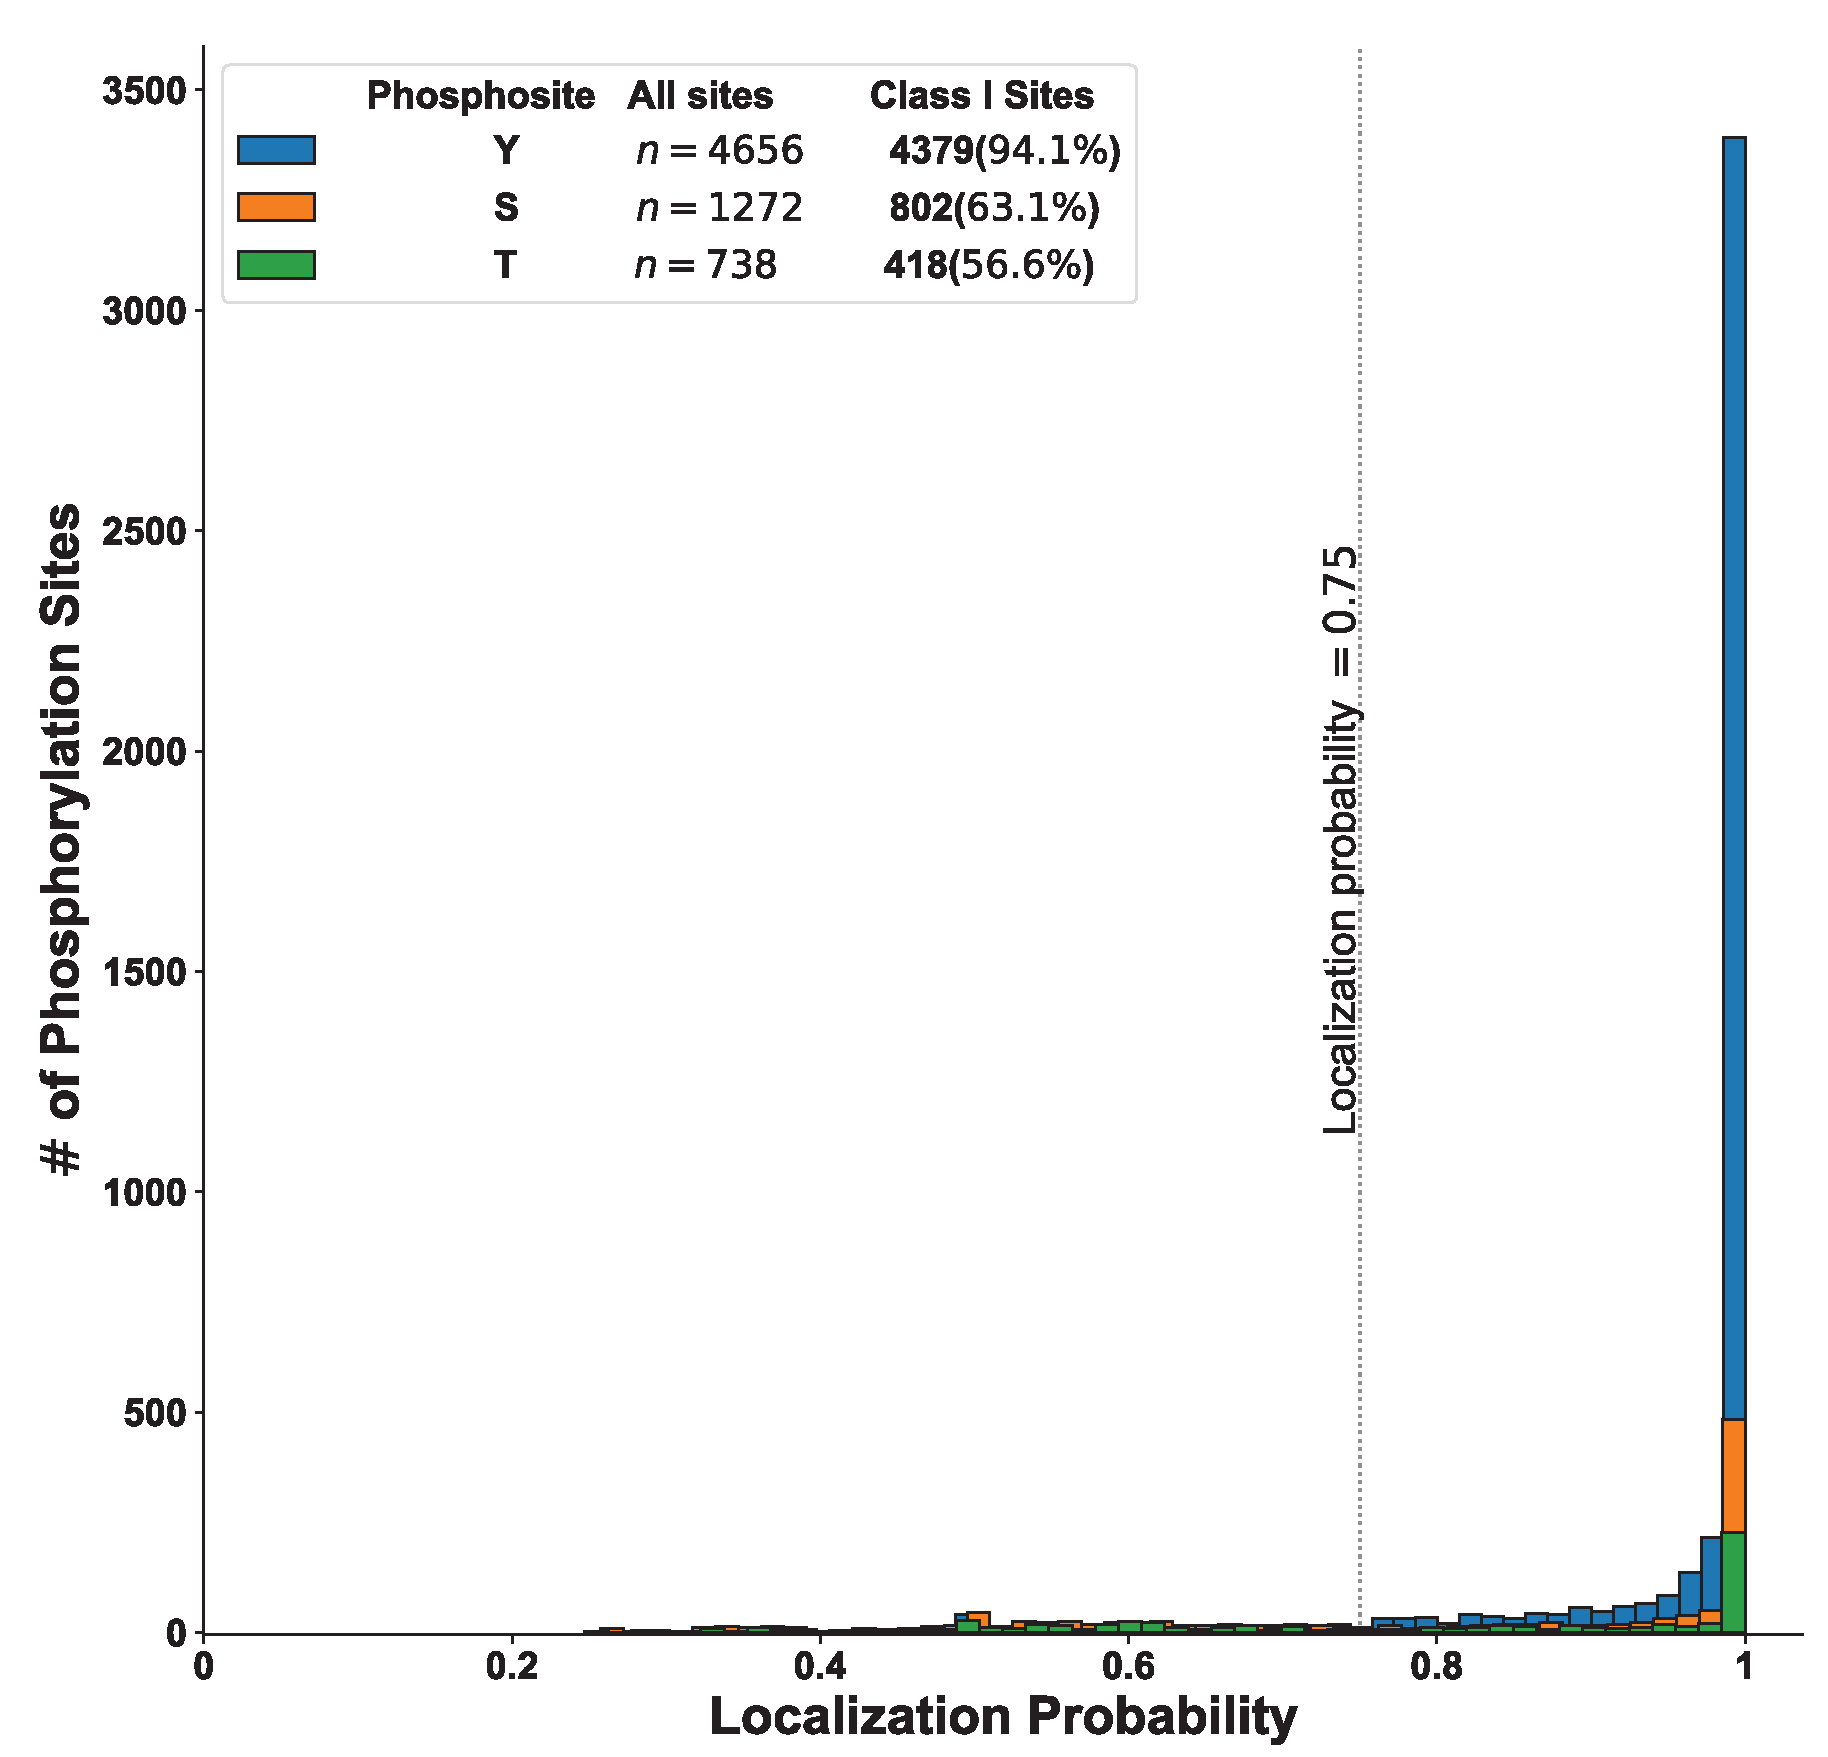
\includegraphics[width=175mm]{figures/supplements/locprob.pdf}
\caption{A histogram with depicting all PSMs from all experiments containing at least one phosphorylated serine (S), threonine (T), or tyrosine (Y) amino acid as a function of localization probability ($n_{\text{bins}} = 75$). The total number and number of Class I (localization probability $>0.75$) phosphorylation sites for each amino acid are noted in the Figure Legend.}\label{locprob}
\end{figure}

\begin{figure}
\centering
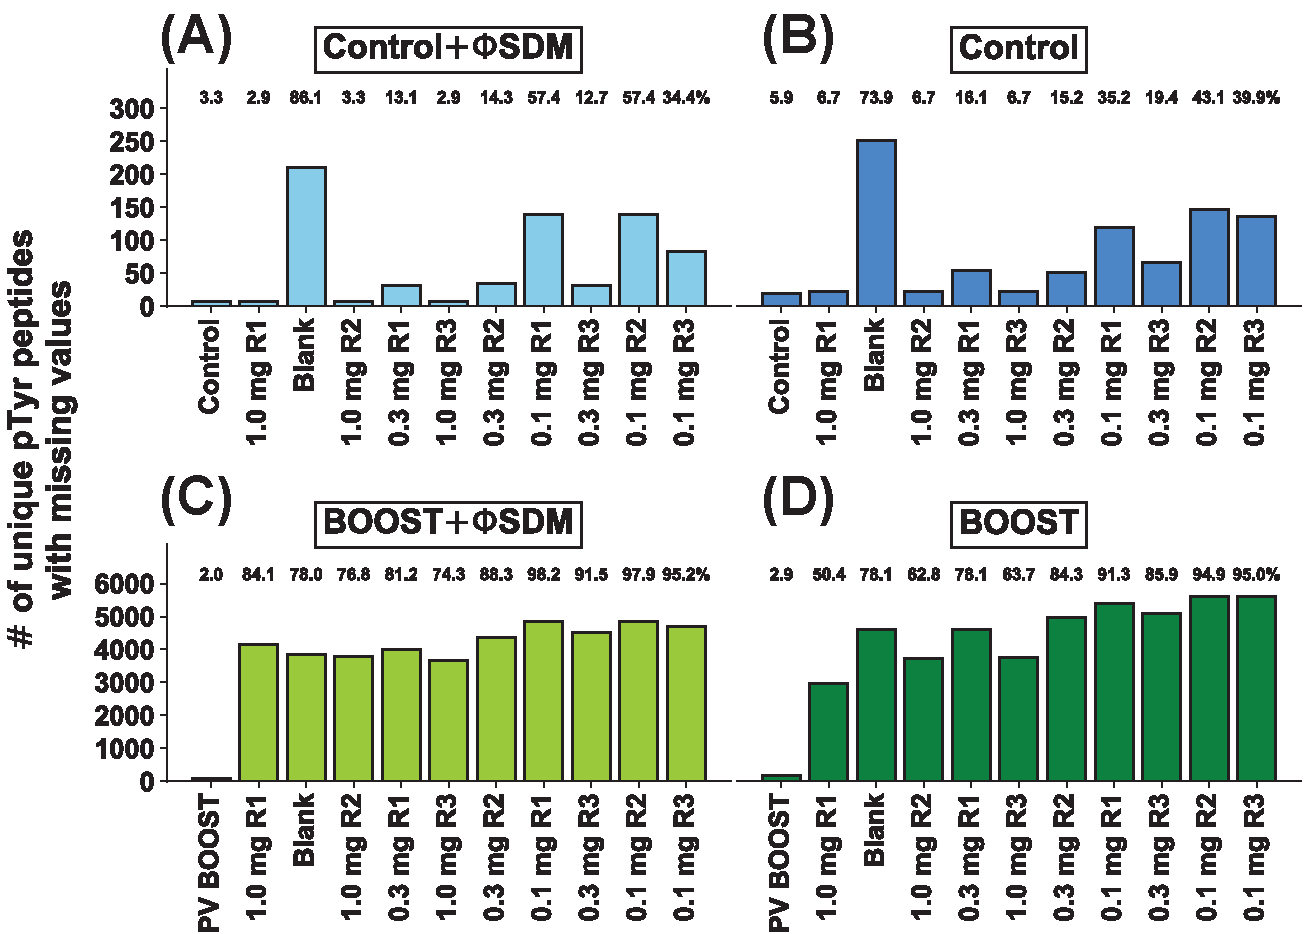
\includegraphics[width=150mm]{figures/supplements/nancounts.pdf}
\caption{Disabling $\Phi$SDM reduces the proportion of missing values in BOOST and $1.0$ mg Control experiments. The number of missing values in each TMT channel for the (A) $1.0$ mg Control experiment with $\Phi$SDM enabled, (B) $1.0$ mg Control experiment with $\Phi$SDM disabled, (C) BOOST experiment with $\Phi$SDM enabled, (D) BOOST experiment with $\Phi$SDM disabled. The percentage of missing values in each TMT channel is indicated above each bar.}
\label{nancounts}
\end{figure}


\begin{figure}
\centering
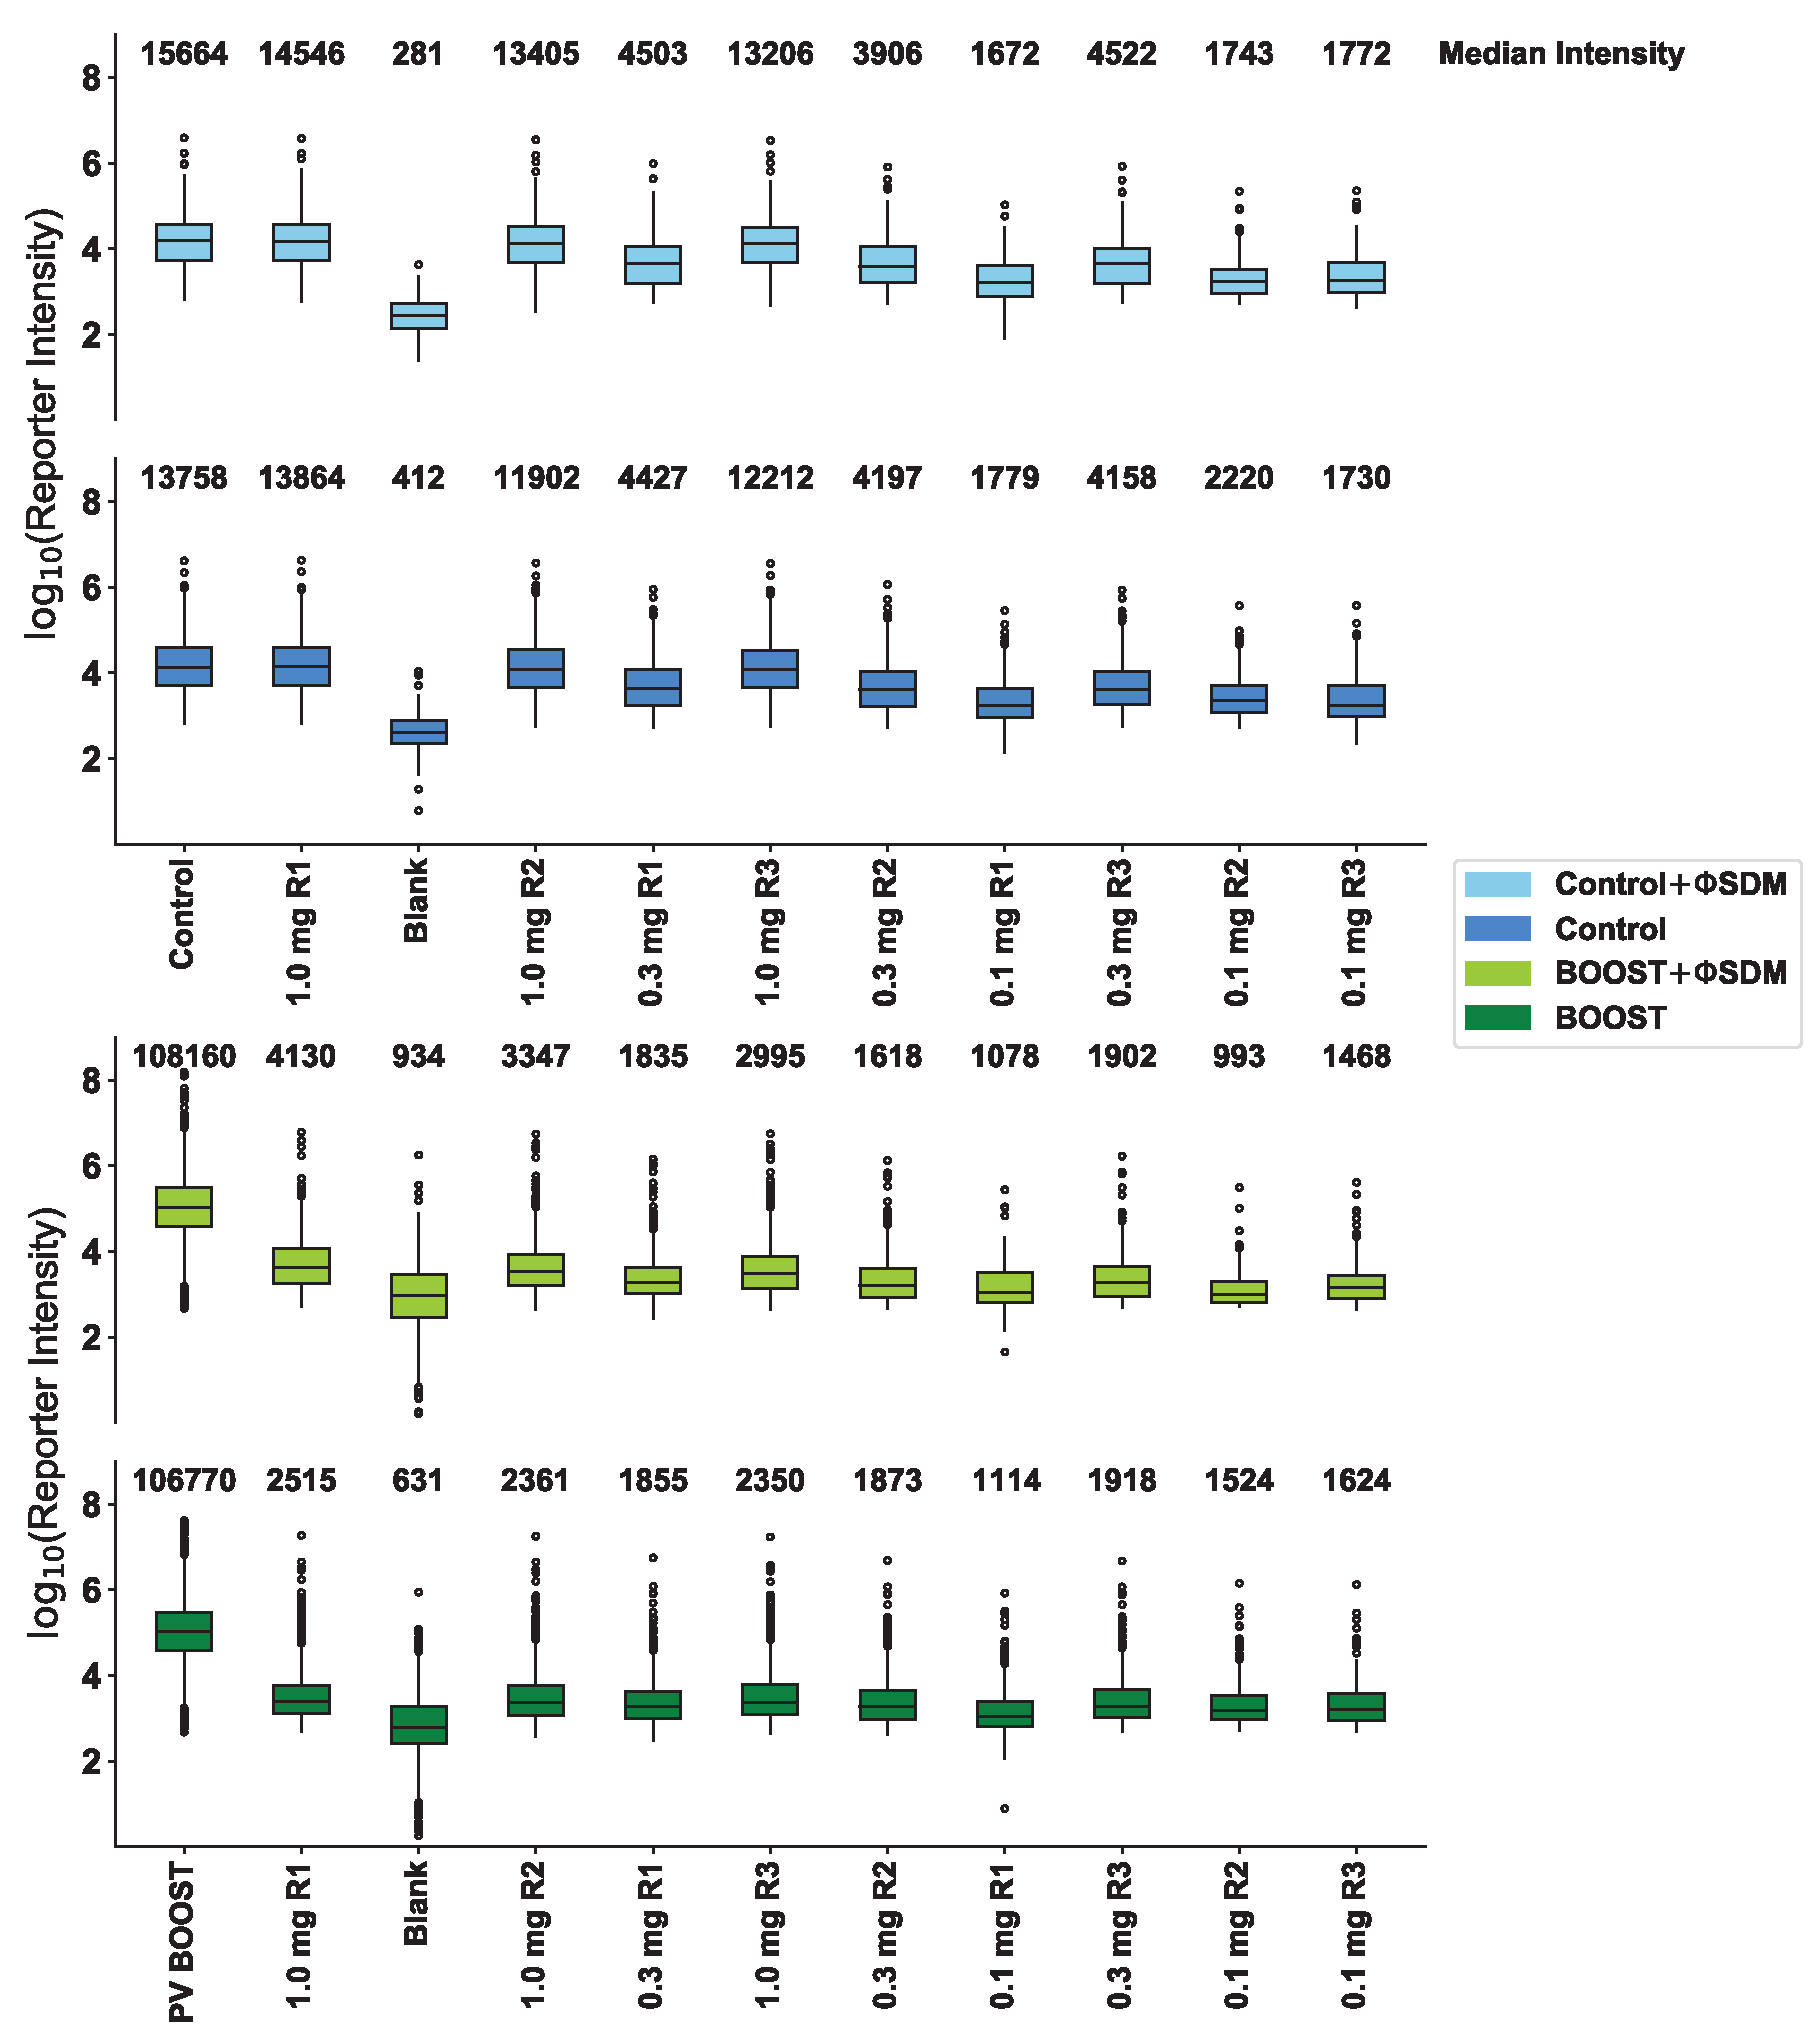
\includegraphics[width=150mm]{figures/supplements/intensity_plots.pdf}
\caption{Box-and-whisker plots showing the $\log_{10}$ transformed reporter intensities for each TMT mix and each condition. Non-transformed, median intensities are displayed above each box-and-whisker plot.}\label{intensity_plots}
\end{figure}

\clearpage

\begin{figure}
\centering
\includegraphics[width=175mm]{figures/supplements/mg1_repmean.pdf}
\caption{Comparison between the reporter ion intensity values and the mean value  for a given pTyr peptide PSM with no missing values in the $1.0$ mg condition of each experiment. The $\log_{10}($Geometric Mean$)$ is on the $x$-axis, while each replicate intensity value is on the $y$-axis. The legend shows the line of best fit as determined by simple linear regression\cite{grus2019data}, and the experiment is noted on the right side of each row.  }\label{mg1_repmean}
\end{figure}

\clearpage

\begin{figure}
\centering
\includegraphics[width=175mm]{figures/supplements/mg03_repmean.pdf}
\caption{Comparison between the reporter ion intensity values and the mean value  for a given pTyr peptide PSM with no missing values in the $0.3$ mg condition of each experiment. The $\log_{10}($Geometric Mean$)$ is on the $x$-axis, while each replicate intensity value is on the $y$-axis. The legend shows the line of best fit as determined by simple linear regression\cite{grus2019data}, and the experiment is noted on the right side of each row. }\label{mg03_repmean}
\end{figure}

\clearpage

\begin{figure}
\centering
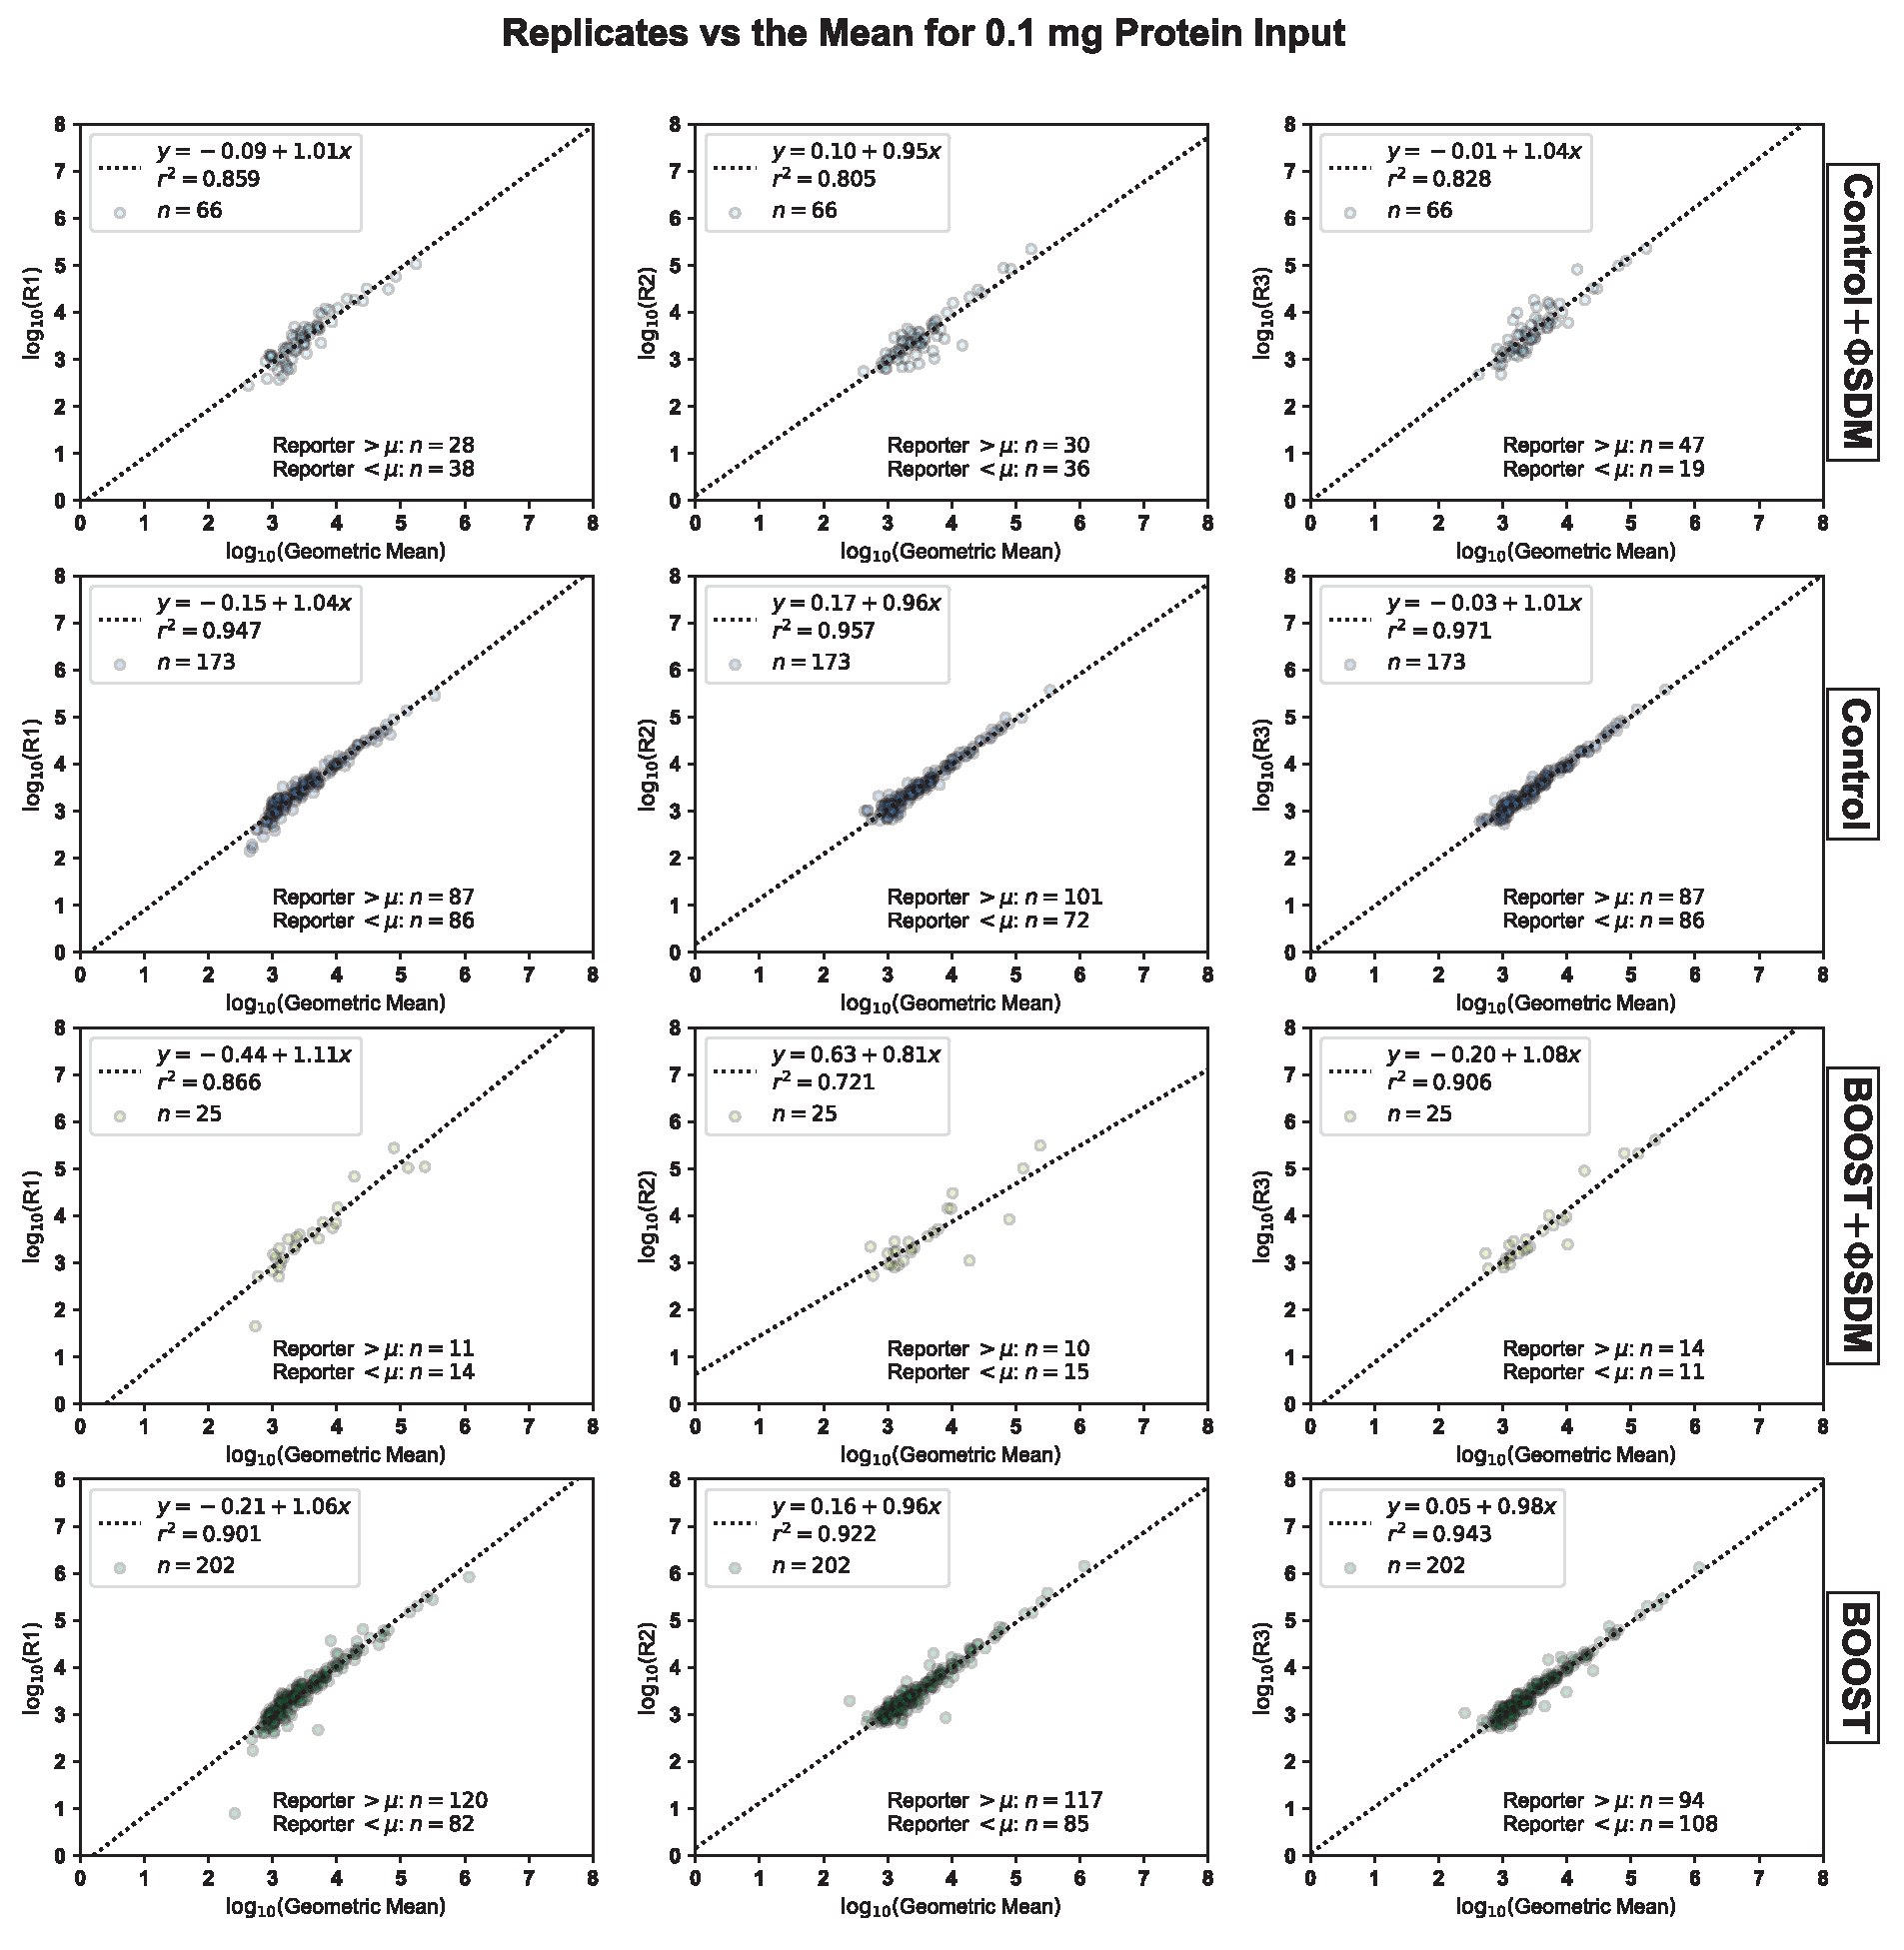
\includegraphics[width=175mm]{figures/supplements/mg01_repmean.pdf}
\caption{Comparison between the reporter ion intensity values and the mean value  for a given pTyr peptide PSM with no missing values in the $0.1$ mg condition of each experiment. The $\log_{10}($Geometric Mean$)$ is on the $x$-axis, while each replicate intensity value is on the $y$-axis. The legend shows the line of best fit as determined by simple linear regression\cite{grus2019data}, and the experiment is noted on the right side of each row. }\label{mg01_repmean}
\end{figure}

\clearpage

\begin{figure}[!t]
\centering
\includegraphics[width=175mm]{figures/supplements/boost_replicate_reprod.pdf}
\caption{Replicate reproducibility is stable when $\Phi$SDM is disabled for low protein input camples in the pervanadate BOOST condition. Evaluation of replicate reproducibility in the BOOST experiment (with $\Phi$SDM disabled) using pairwise comparisons of $\log_2$ transformed abundances for pTyr peptide PSMs with the same charge state and assigned sequence. For each comparison, we show the line of best fit as determined by simple least-squares regression\cite{grus2019data}, the $r^2$ value as an estimate of the quality of the fitted line, and the total number of points ($n$) in each comparison.}\label{boost_replicate_reprod}
\end{figure}

\clearpage

\begin{figure}[t!]
\centering
\includegraphics[width=175mm]{figures/supplements/boostsdm_replicate_reprod}
\caption{Replicate reproducibility is severely degraded when $\Phi$SDM is enabled for low protein input samples in the pervanadate BOOST condition. Evaluation of replicate reproducibility in the BOOST experiment (with $\Phi$SDM enabled) using pairwise comparisons of $\log_2$ transformed abundances for  pTyr peptide PSMs with the same charge state and assigned sequence. For each comparison, we show the line of best fit as determined by simple least-squares regression\cite{grus2019data}, the $r^2$ value as an estimate of the quality of the fitted line, and the total number of points ($n$) in each comparison. }\label{boostsdm_replicate_reprod}
\end{figure}

\clearpage

\begin{figure}[t!]
\centering
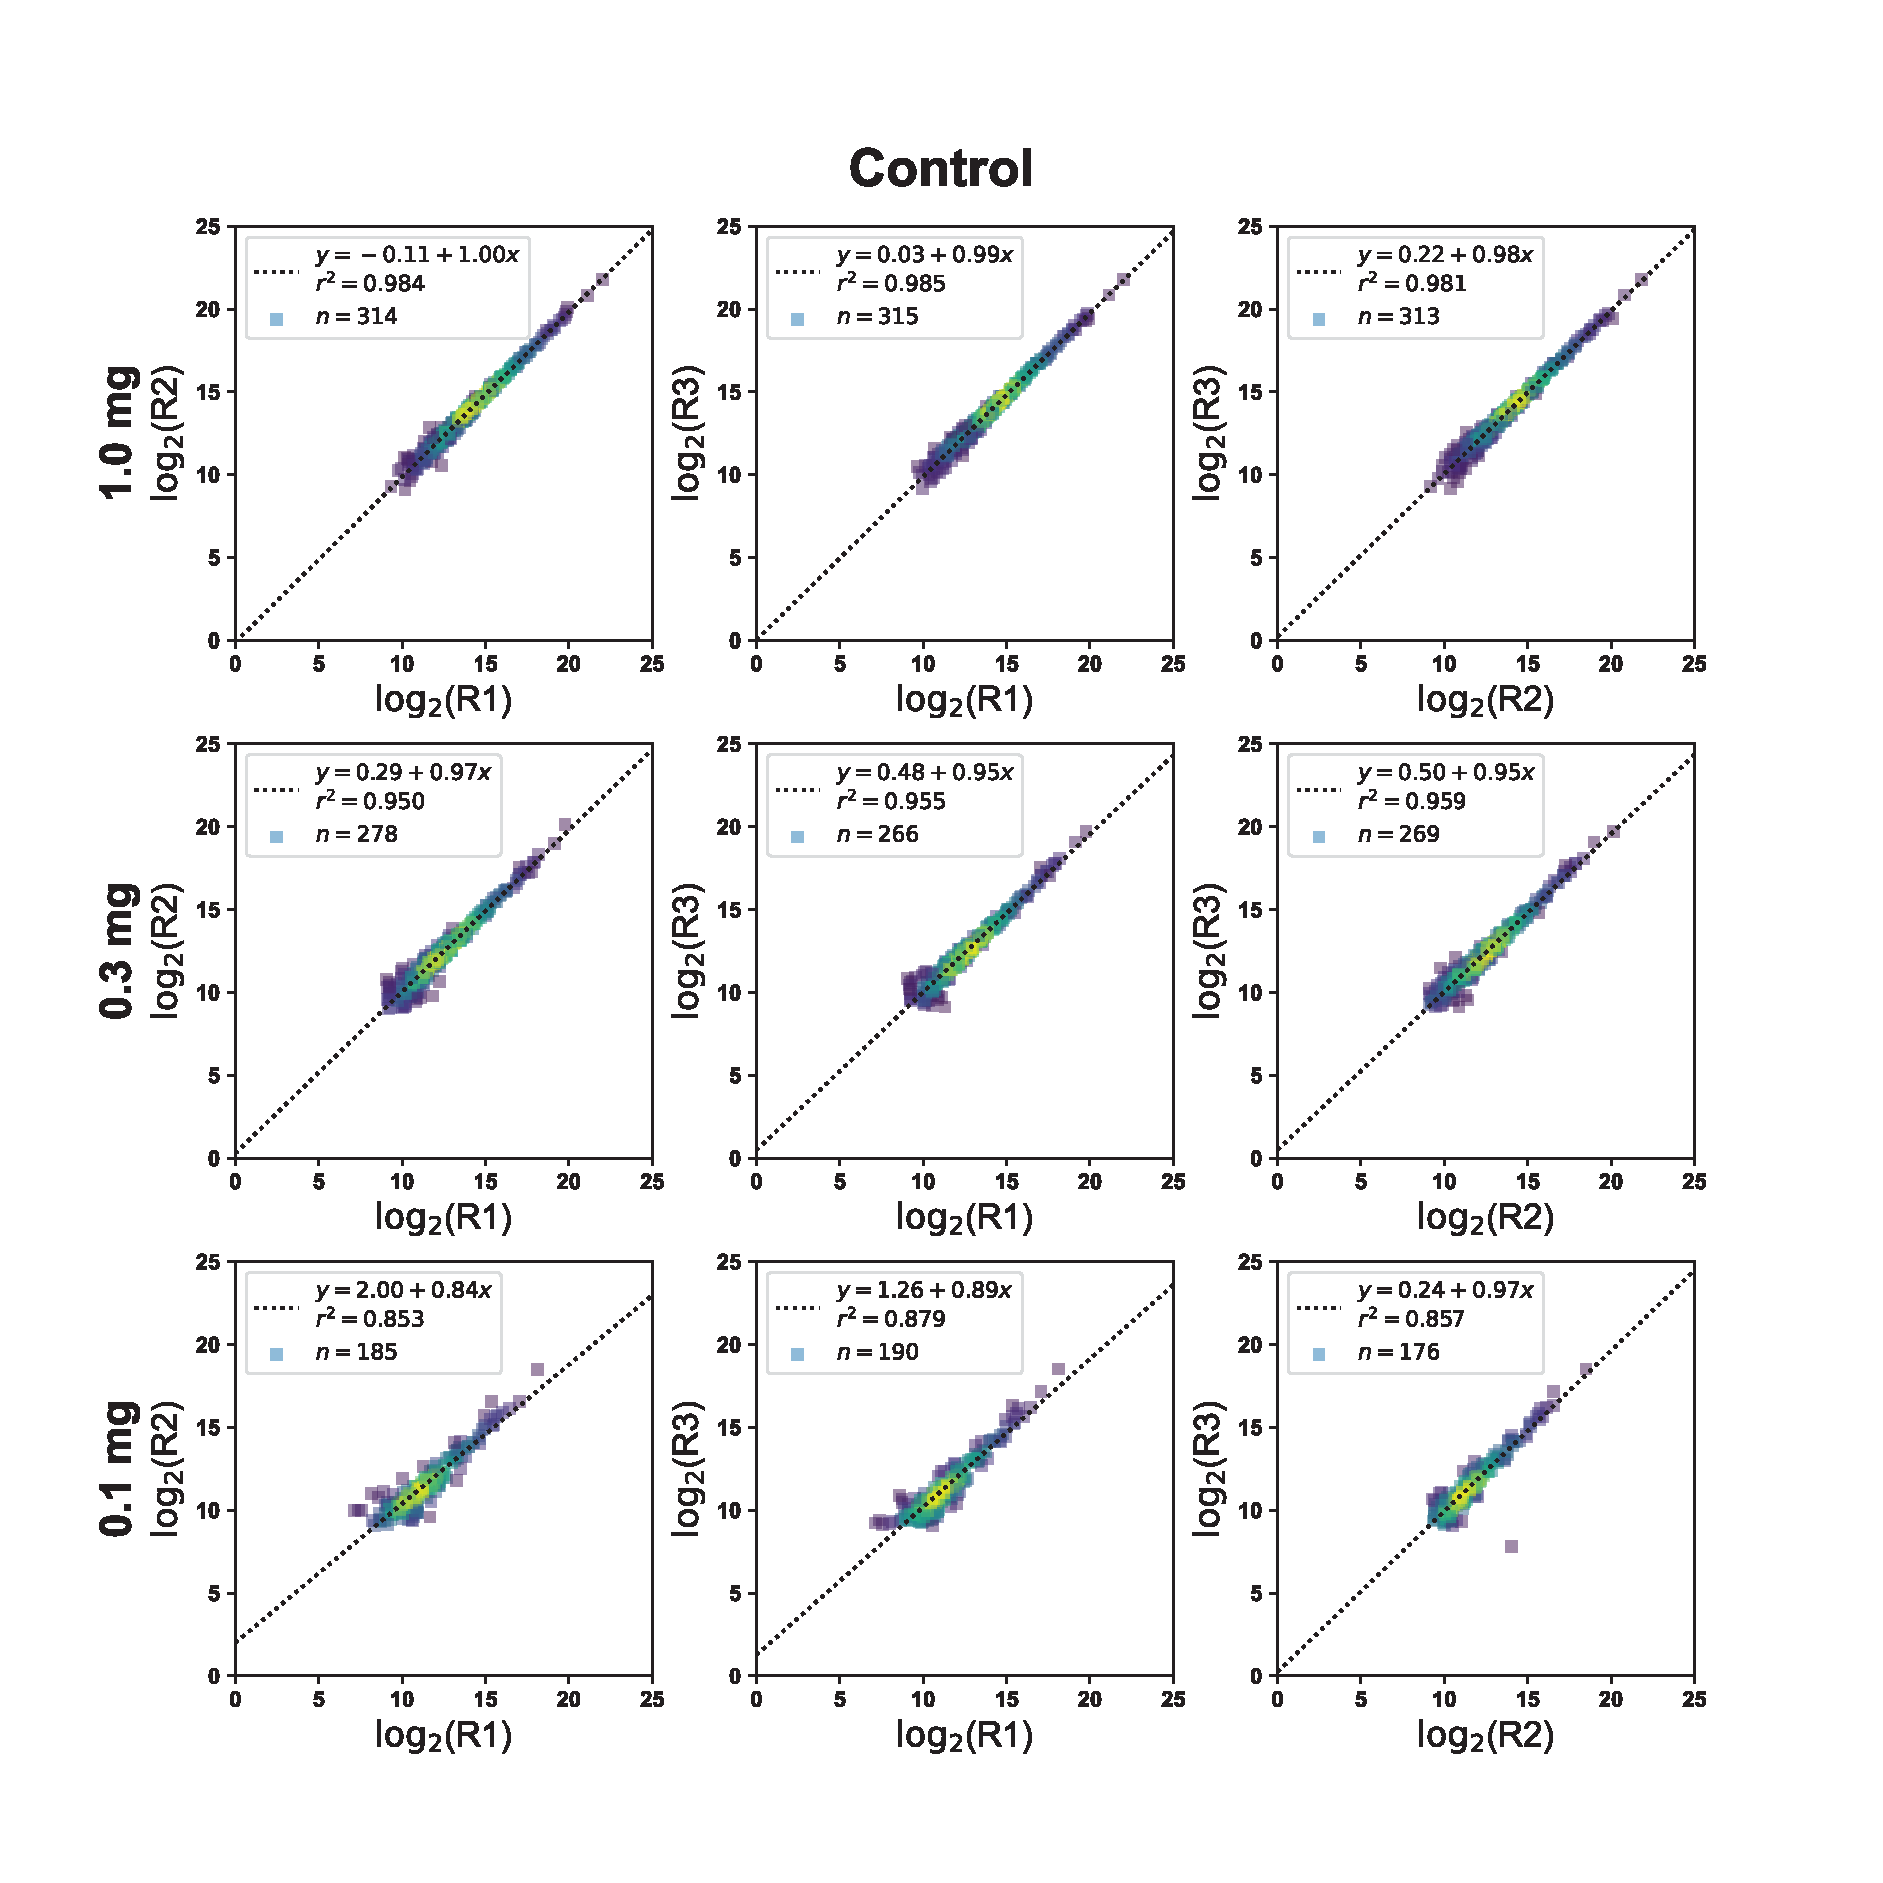
\includegraphics[width=175mm]{figures/supplements/control_replicate_reprod.pdf}
\caption{Replicate reproducibility is stable when $\Phi$SDM is disabled for low protein input camples in the $1.0$ mg Control condition. Evaluation of replicate reproducibility in the $1.0$ mg Control experiment (with $\Phi$SDM disabled) using pairwise comparisons of $\log_2$ transformed abundances for  pTyr peptide PSMs with the same charge state and assigned sequence. For each comparison, we show the line of best fit as determined by simple least-squares regression\cite{grus2019data}, the $r^2$ value as an estimate of the quality of the fitted line, and the total number of points ($n$) in each comparison. }\label{control_replicate_reprod}
\end{figure}

\clearpage

\begin{figure}[t!]
\centering
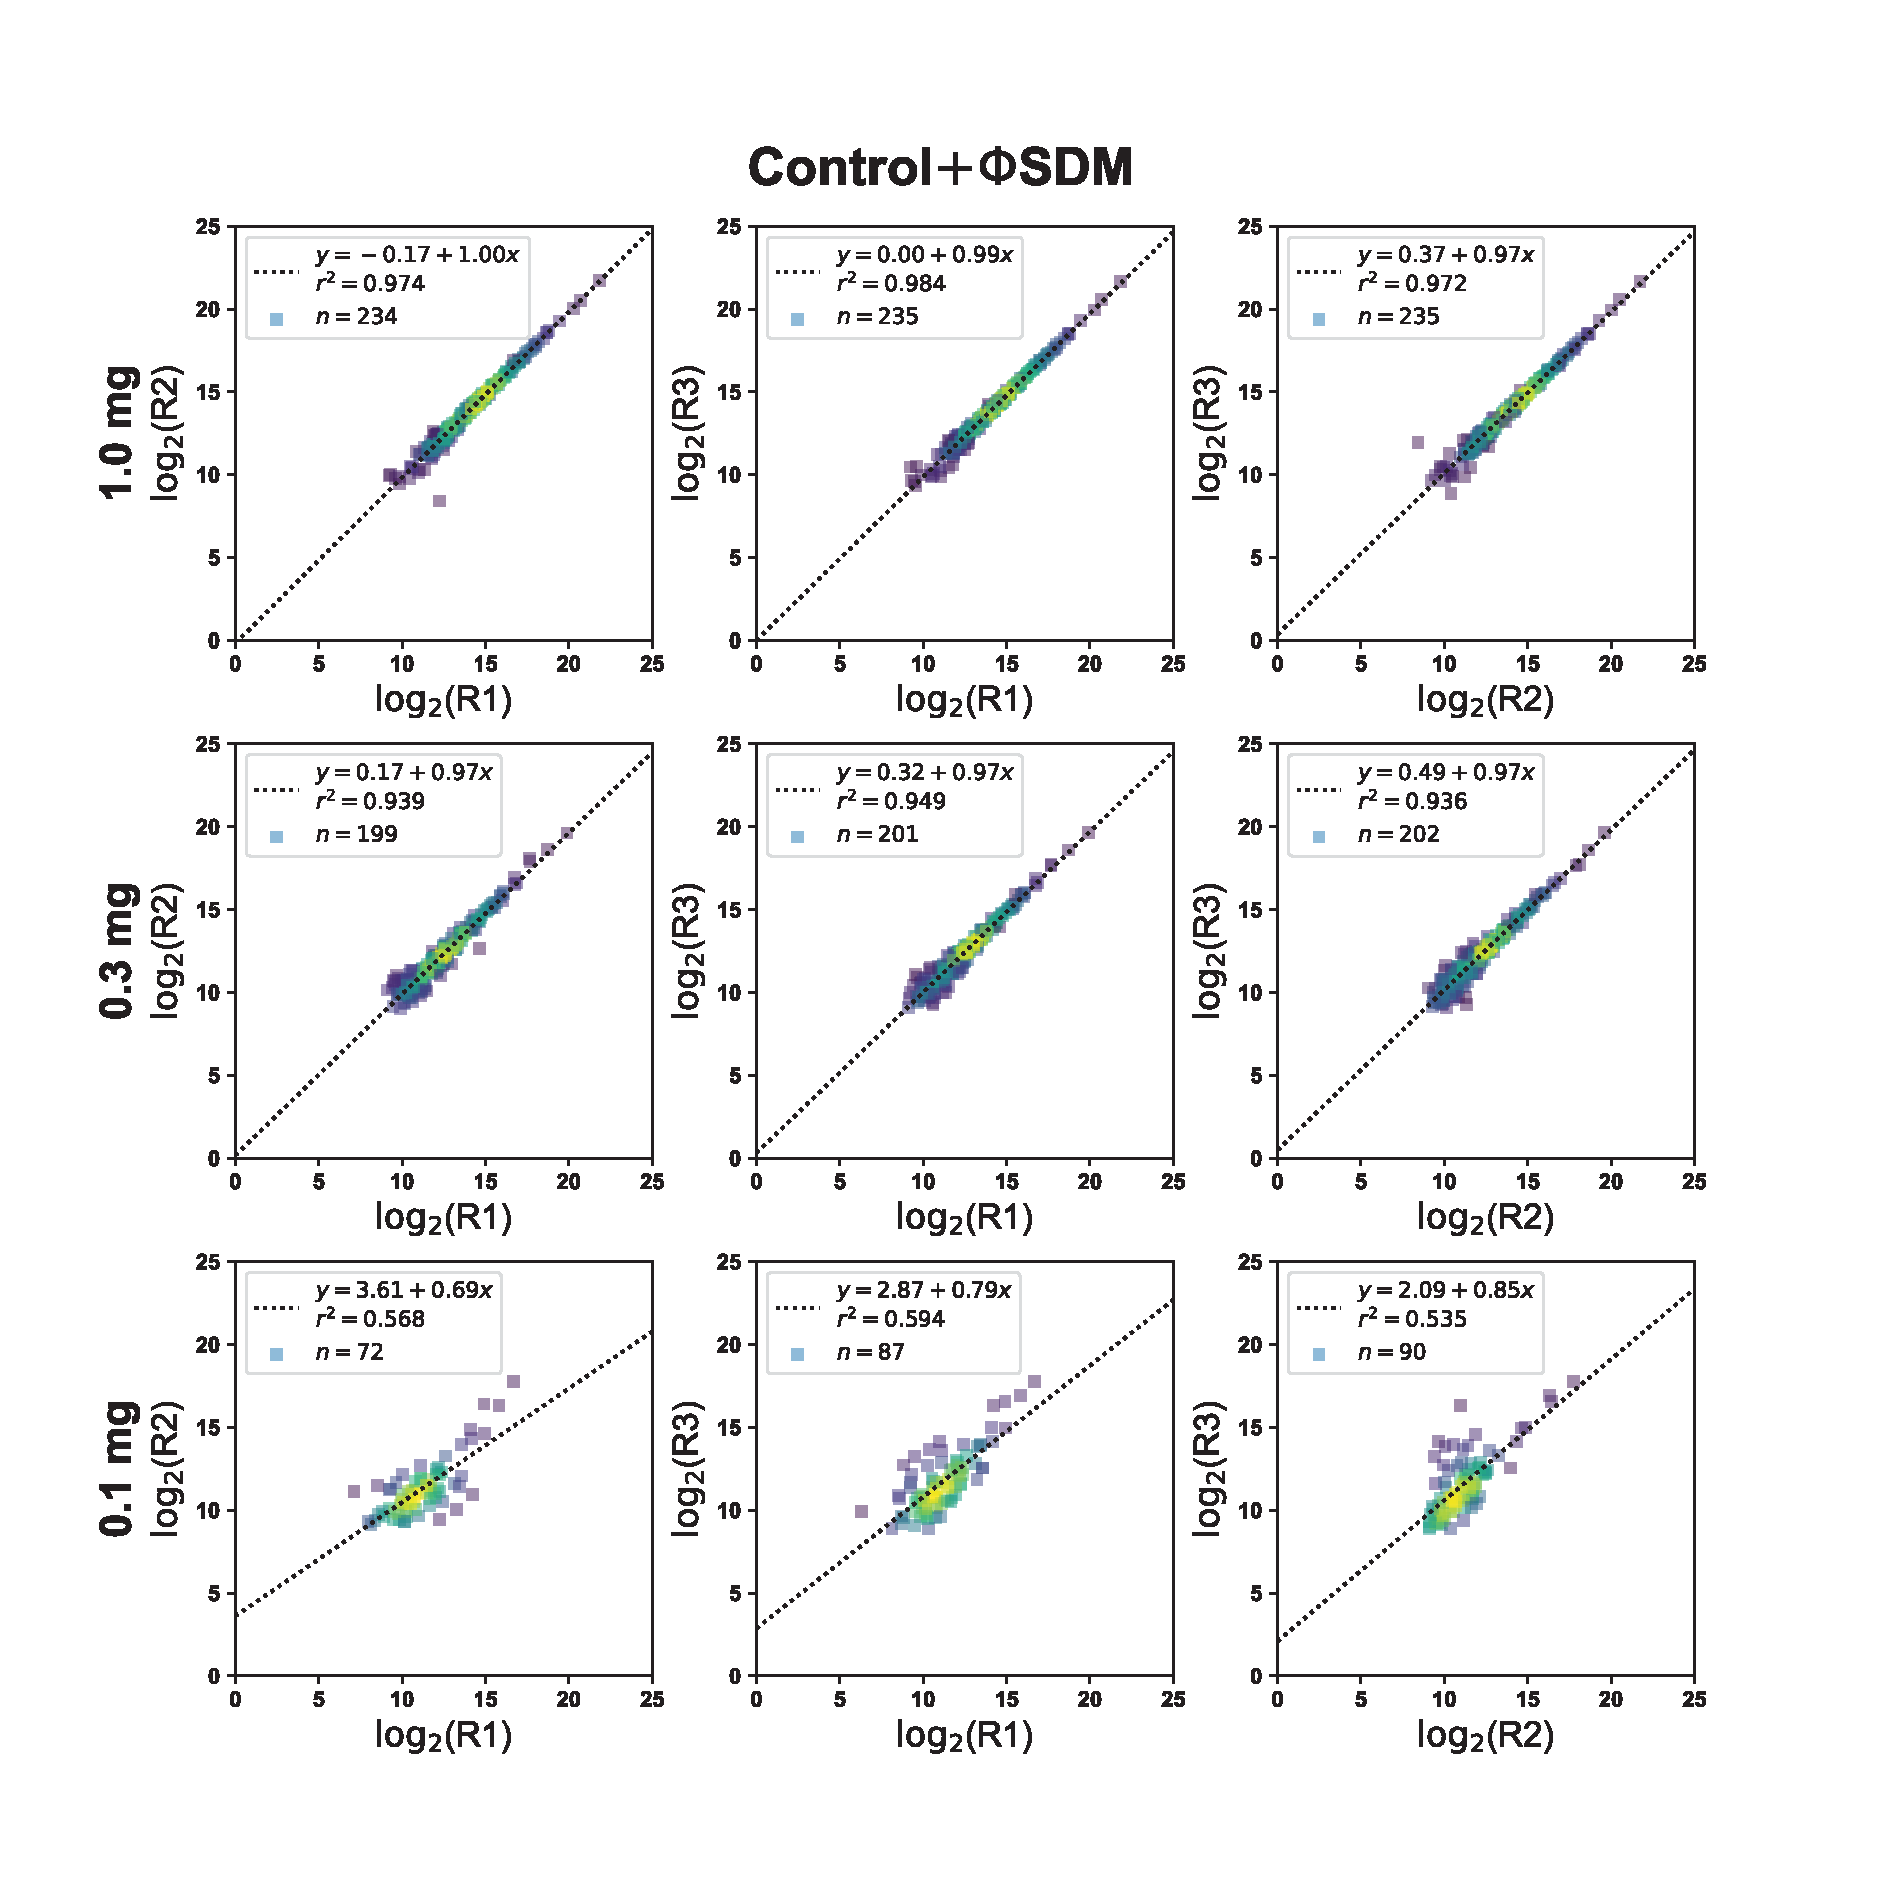
\includegraphics[width=175mm]{figures/supplements/controlsdm_replicate_reprod.pdf}
\caption{Replicate reproducibility is degraded when $\Phi$SDM is enabled for low protein input samples in the $1.0$ mg Contro conditionl. Evaluation of replicate reproducibility in the $1.0$ mg experiment (with $\Phi$SDM enabled) using pairwise comparisons of $\log_2$ transformed abundances for  pTyr peptide PSMs with the same charge state and assigned sequence. For each comparison, we show the line of best fit as determined by simple least-squares regression\cite{grus2019data}, the $r^2$ value as an estimate of the quality of the fitted line, and the total number of points ($n$) in each comparison. }\label{controlsdm_replicate_reprod}
\end{figure}

\clearpage

\begin{figure}[t!]
\centering
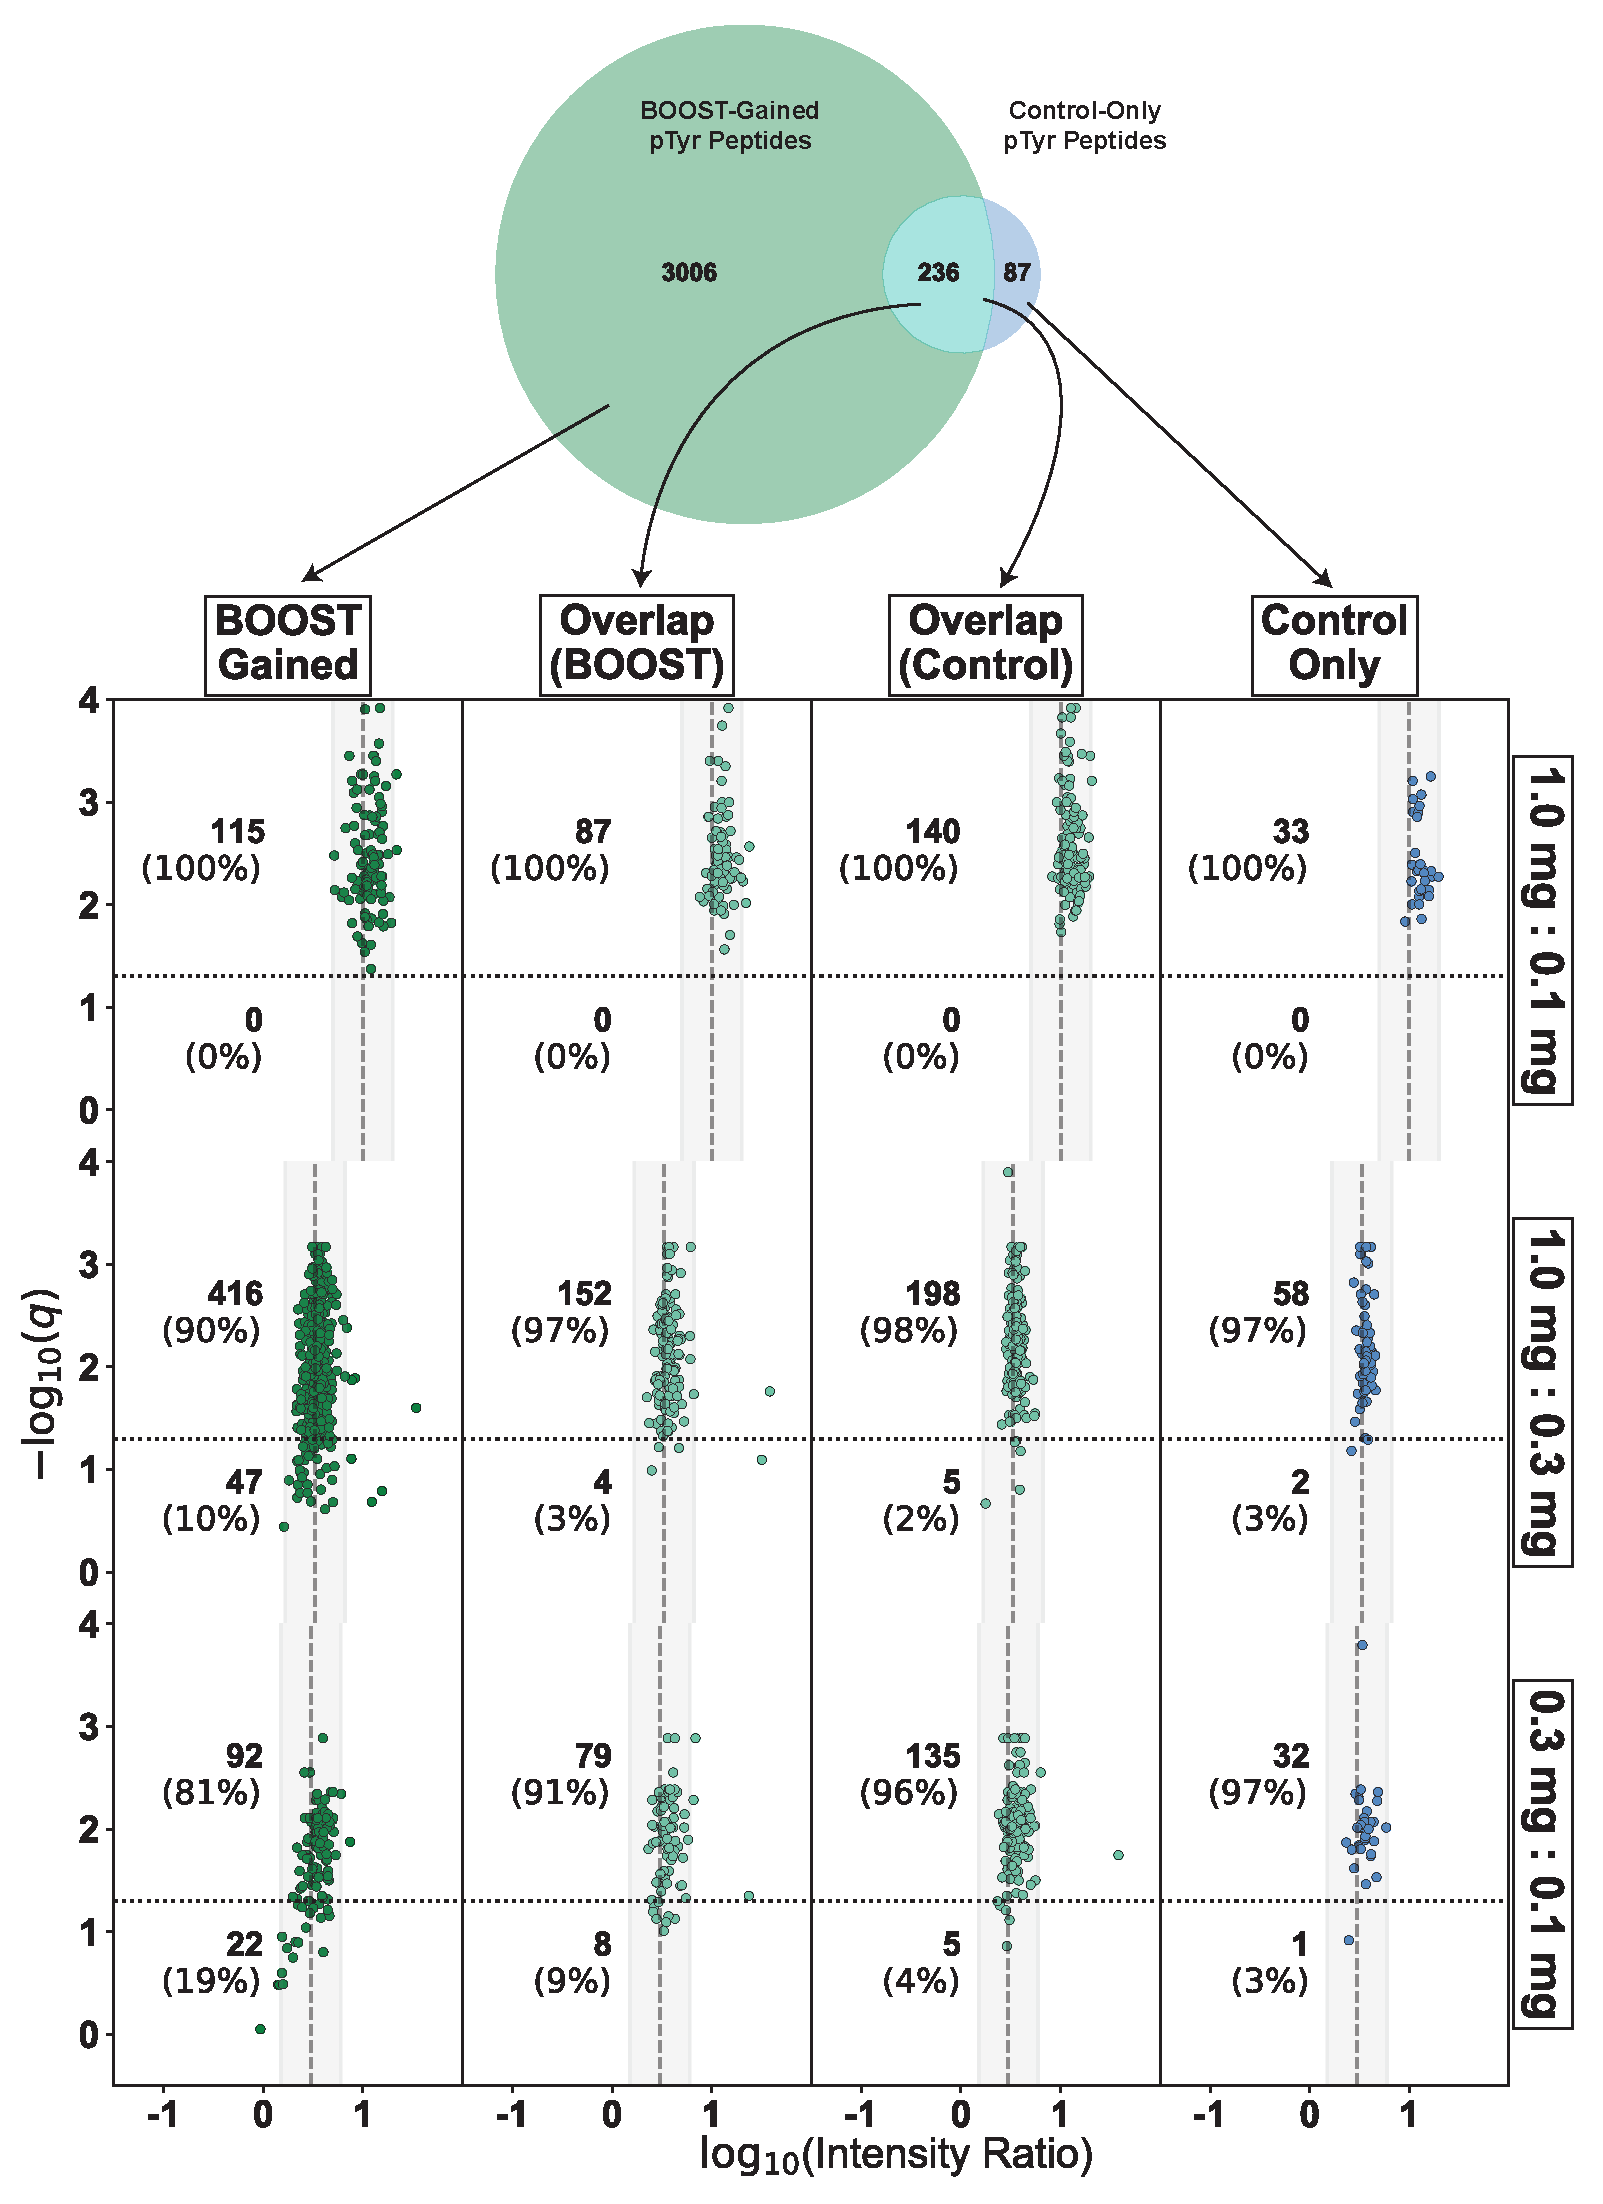
\includegraphics[width=135mm]{figures/supplements/boost_control_gained_qvolcanoes.pdf}
\caption{With $\Phi$SDM disabled, the pervanadate BOOST channel dramatically increases the number of unique pTyr peptide PSMs observed as compared to a $1.0$ mg Control channel. A Venn diagram showing the overlap of unique pTyr peptide PSMs between the BOOST and $1.0$ mg Control experiments (with $\Phi$SDM disabled). Volcano plots show $-\log_{10}(q\text{-value})$ as a function of $\log_{10}(\text{Intensity Ratio})$ for unique pTyr peptide PSMs from groups show in the Venn diagram. For the overlapping section, volcano plots were created using data from both the BOOST experiment and the control experiment acquired with $\Phi$SDM disabled. }\label{boost_control_gained_qvolcanoes}
\end{figure}


%\addtocounter{figure}{-1}
%\begin{figure}[t!]
%\caption{With $\Phi$SDM disabled, the pervanadate BOOST channel dramatically increases the number of unique pTyr peptides observed as compared to a $1.0$ mg Control channel. A Venn diagram showing the overlap of unique pTyr peptides between the BOOST and $1.0$ mg Control experiments (with $\Phi$SDM disabled). Volcano plots show $-\log_{10}(q\text{-value})$ as a function of $\log_{10}(\text{Intensity Ratio})$ for unique pTyr peptides from the BOOST experiment only (``BOOST Gained"), BOOST and Control overlap (from the BOOST experiment; ``BOOST $\cap$ Control"), Control and BOOST overlap (from the Control experiment; ``Control $\cap$ BOOST"), and Control experiment only (``Control Only"). }\label{boost_control_gained_qvolcanoes}
%\end{figure}

\clearpage

\begin{figure}[t!]
\centering
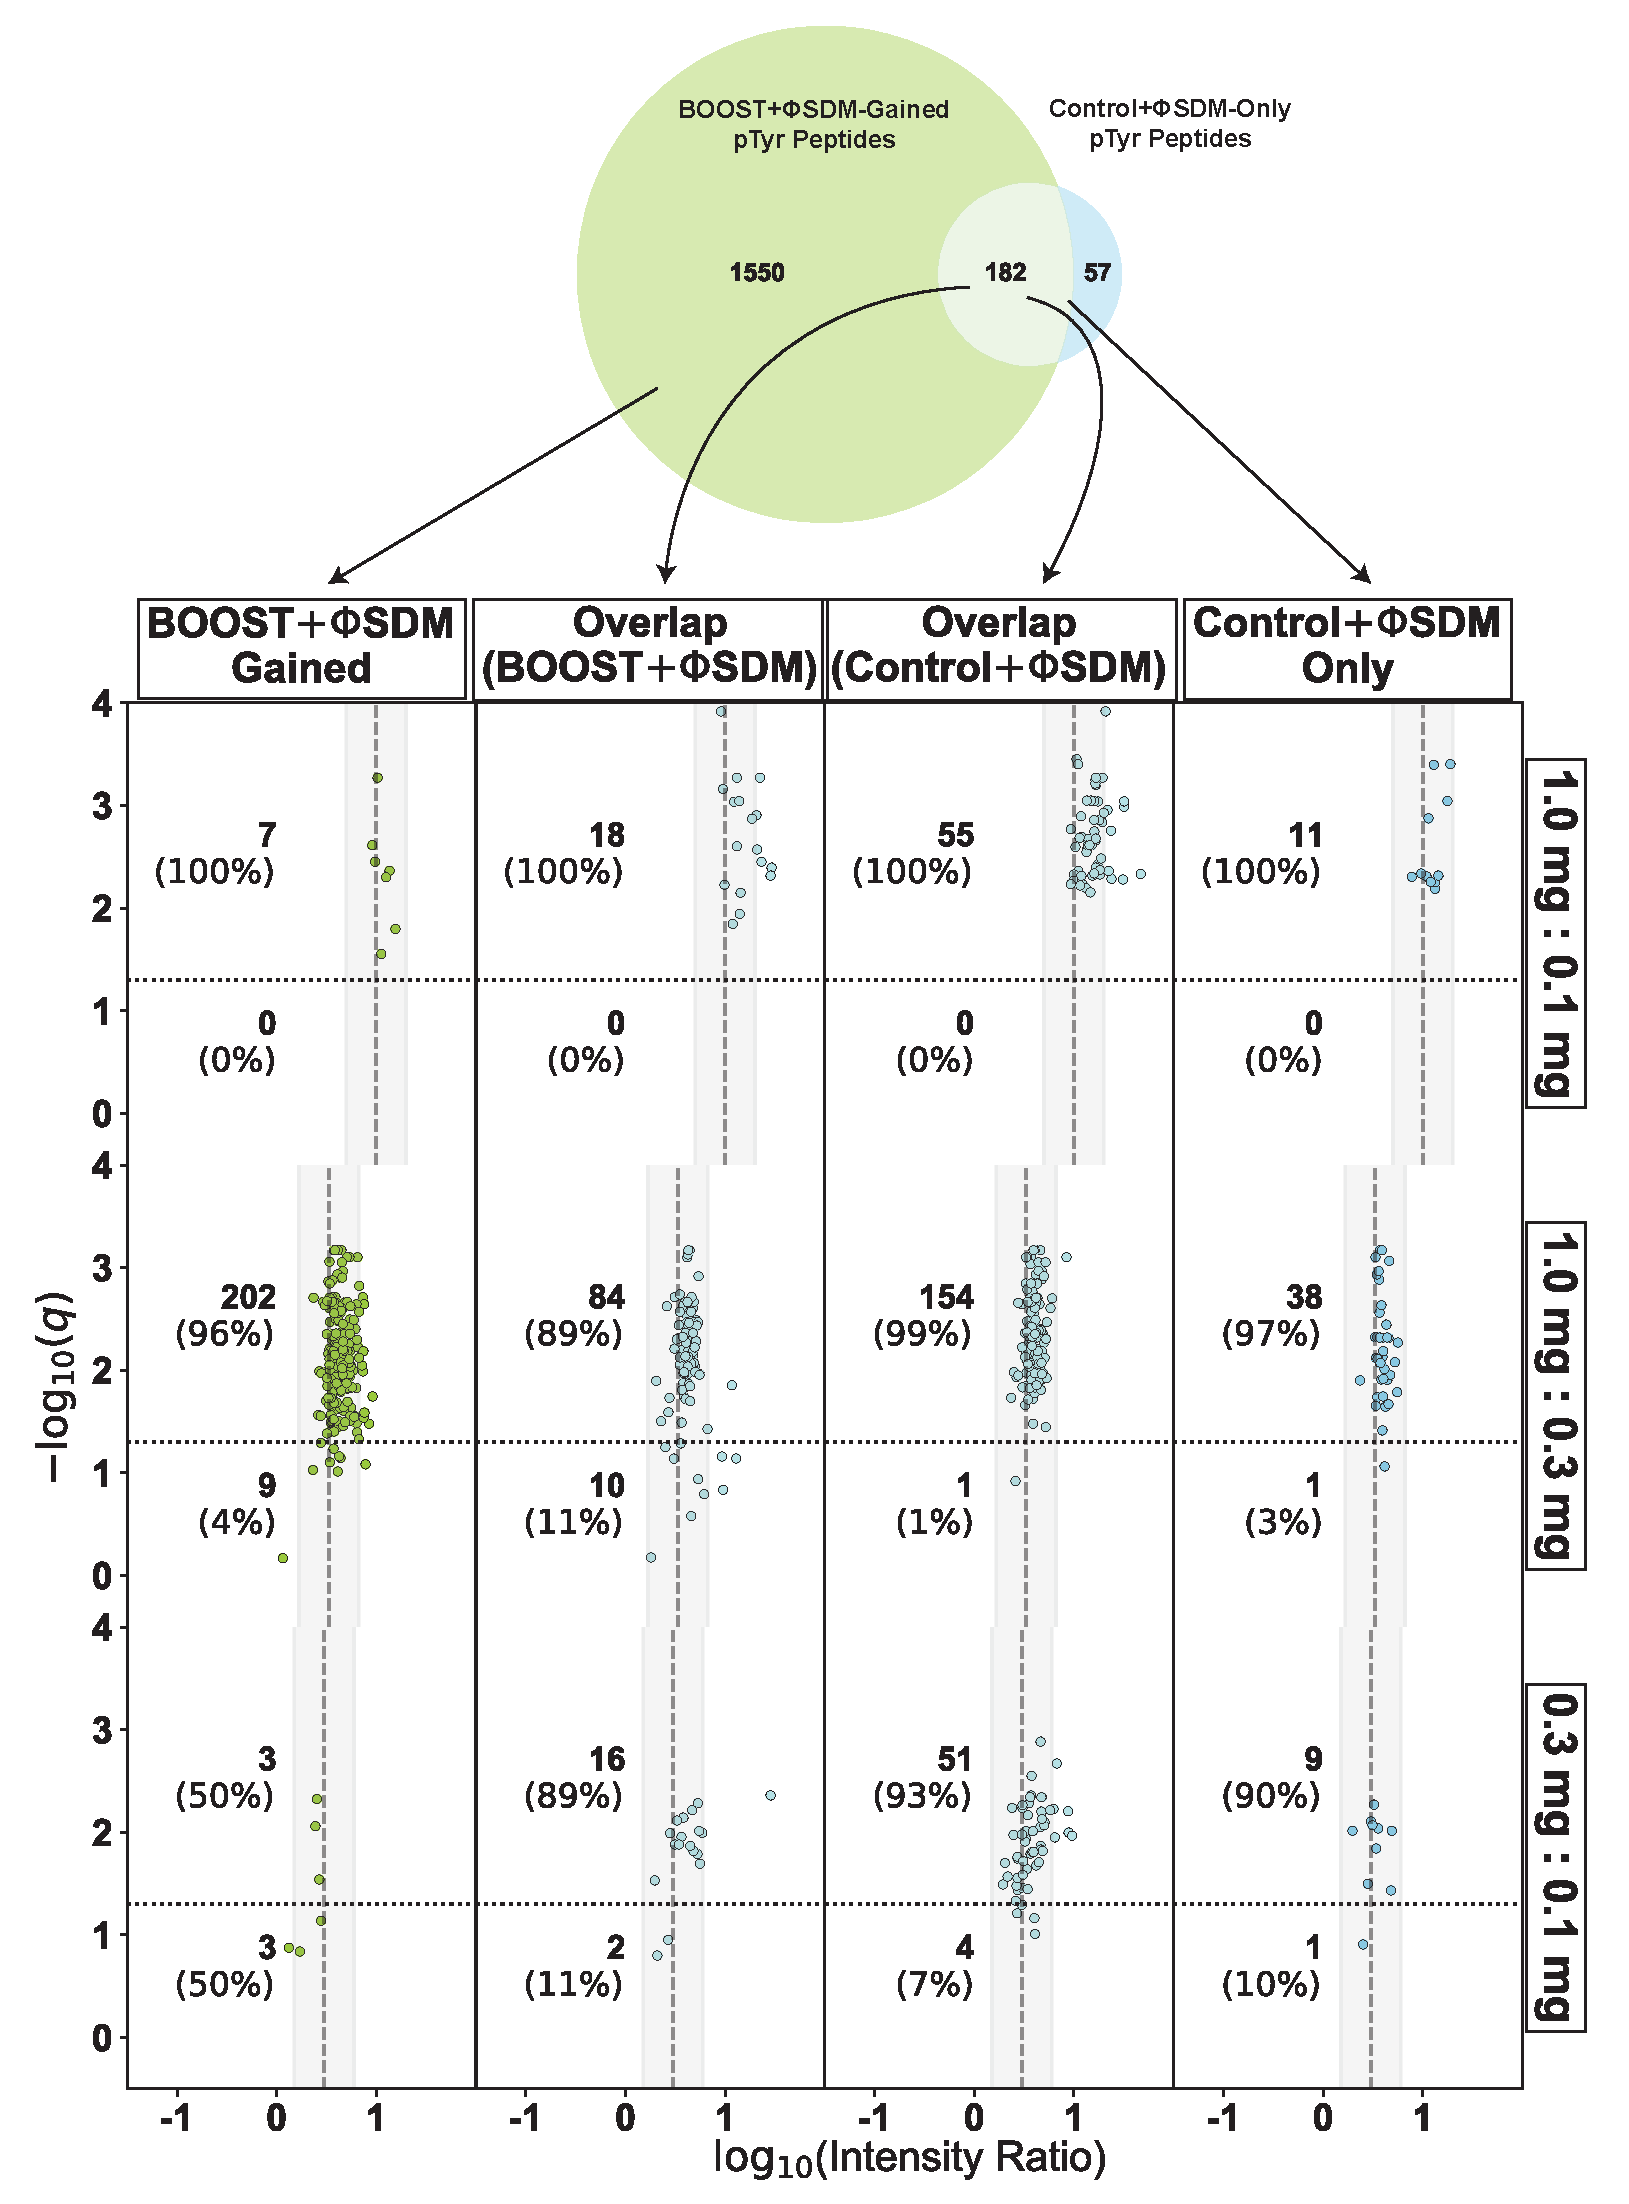
\includegraphics[width=135mm]{figures/supplements/boostsdm_controlsdm_gained_qvolcanoes.pdf}
\caption{The pervanadate BOOST channel increases the number of unique pTyr peptide PSMs observed when $\Phi$SDM is enabled, although few peptide PSMs are observed in low abundance samples. A Venn diagram showing the overlap of unique pTyr peptide PSMs between the BOOST$+\Phi$SDM and $1.0$ mg Control$+\Phi$SDMl experiments. Volcano plots show $-\log_{10}(q\text{-value})$ as a function of $\log_{10}(\text{Intensity Ratio})$ for unique pTyr peptide PSMs from groups show in the Venn diagram. For the overlapping section, volcano plots were created using data from both the BOOST experiment and the control experiment acquired with $\Phi$SDM enabled. }\label{boostsdm_controlsdm_gained_qvolcanoes}
\end{figure}

%\addtocounter{figure}{-1}
%\begin{figure}[t!]
%\caption{The pervanadate BOOST channel increases the number of unique pTyr peptides observed when $\Phi$SDM is enabled, although few peptides are observed in low abundance samples. A Venn diagram showing the overlap of unique pTyr peptides between the BOOST$+\Phi$SDM and $1.0$ mg Contro$+\Phi$SDMl experiments. Volcano plots show $-\log_{10}(q\text{-value})$ as a function of $\log_{10}(\text{Intensity Ratio})$ for unique pTyr peptides from the BOOST$+\Phi$SDM experiment only (``BOOST$+\Phi$SDM Gained"), BOOST$+\Phi$SDM and Control$+\Phi$SDM overlap (from the BOOST$+\Phi$SDM experiment; ``BOOST$+\Phi$SDM $\cap$ Contro$+\Phi$SDMl"), Contro$+\Phi$SDMl and BOOST$+\Phi$SDM overlap (from the Control$+\Phi$SDM experiment; ``Control$+\Phi$SDM $\cap$ BOOST$+\Phi$SDM"), and Control$+\Phi$SDM experiment only (``Control$+\Phi$SDM Only"). }\label{boostsdm_controlsdm_gained_qvolcanoes}
%\vspace*{5cm}
%\end{figure}

\clearpage

\begin{figure}[t!]
\centering
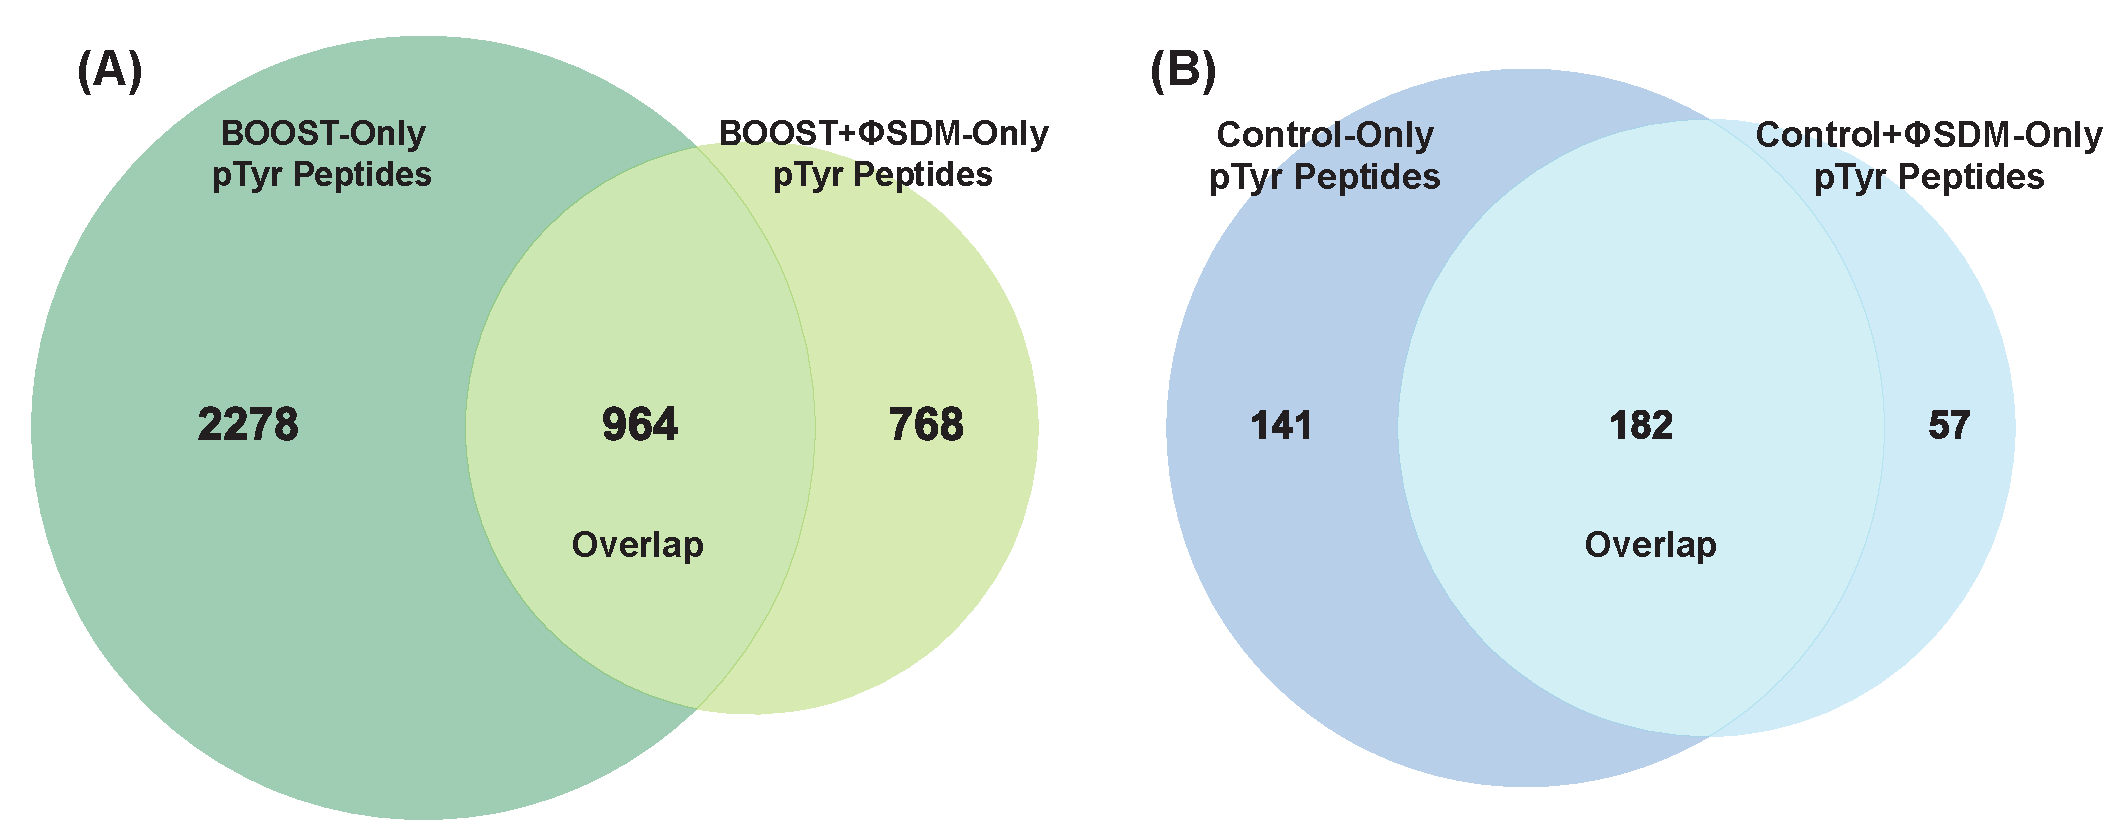
\includegraphics[width=165mm]{figures/supplements/set_overlap_2.pdf}
\caption{Enabling $\Phi$SDM results in lower yield in both pervanadate BOOST and $1.0$ mg Control conditions. Venn diagrams showing the number of unique pTyr peptide PSMs observed when $\Phi$SDM is enabled or disabled using (A) pervanadate BOOST samples, and (B) $1.0$ mg Control samples.}\label{set_overlap_2}
\end{figure}

\clearpage

\begin{figure}[t!]
\centering
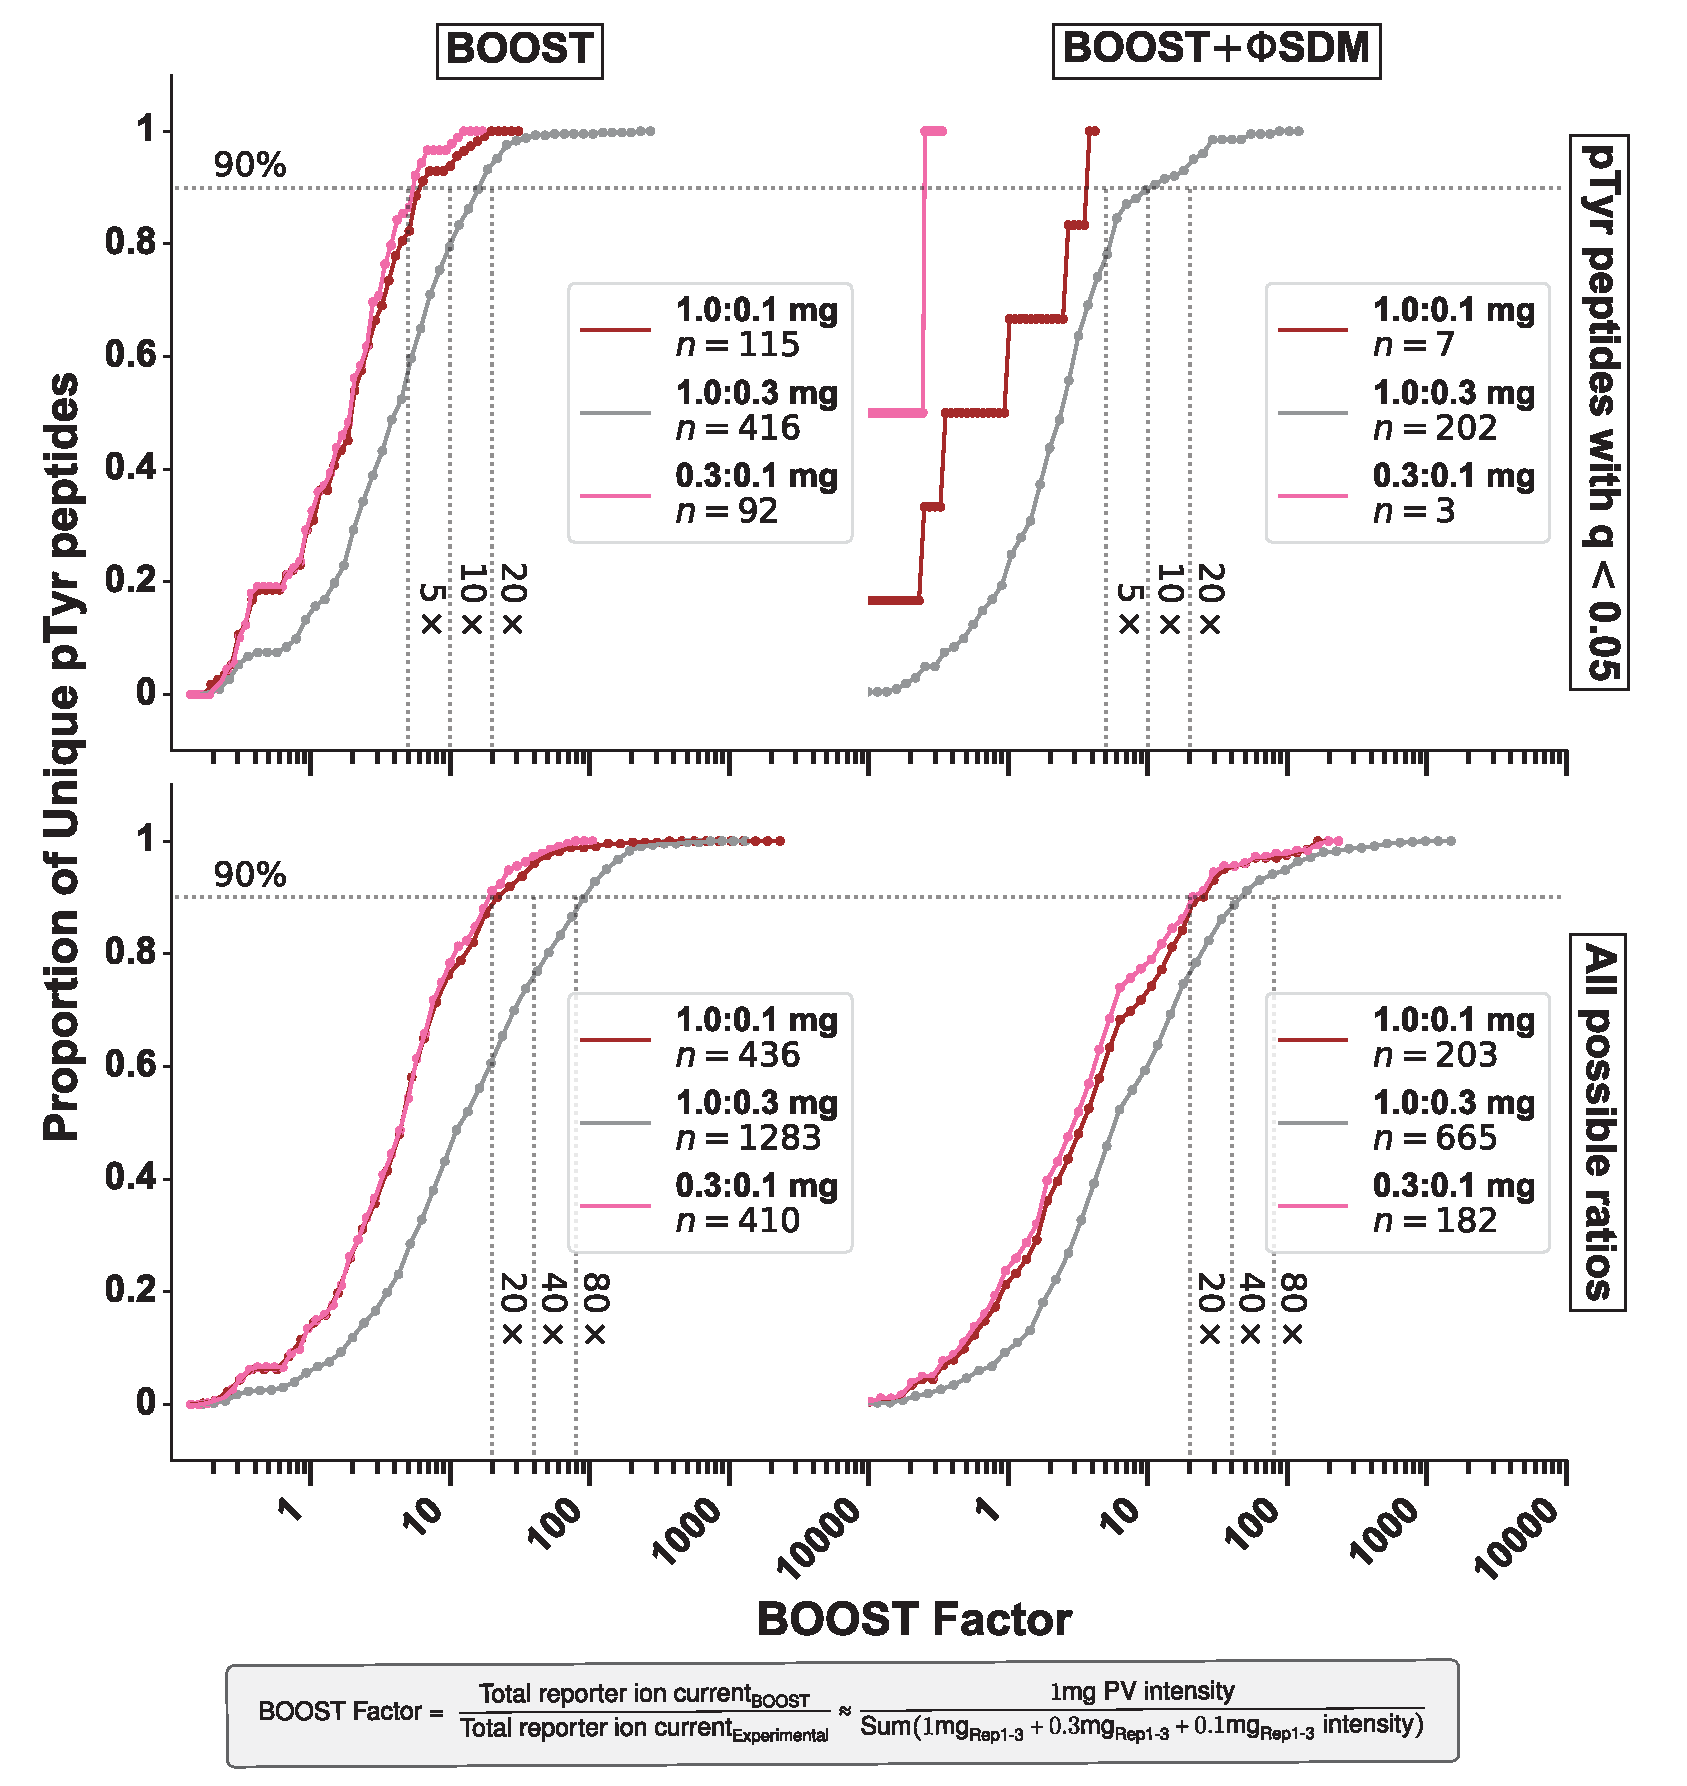
\includegraphics[width=165mm]{figures/supplements/boost_factor_cdfs.pdf}
\caption{Enabling $\Phi$SDM decreases quantitation depth, particularly in low abundance samples. Cumulative distribution of BOOST factors for unique pTyr peptides identified in the pervanadate BOOST experiments with $\Phi$SDM disabled or with $\Phi$SDM enabled for pTyr peptides with a statistically significant ratio ($q<0.05$) or for all calculable ratios. For each cumulative distribution, the range of BOOST factors are split into $50$ bins of equal size on a $\log_{10}$ scale. }\label{boost_factor_cdfs}
\end{figure}

\clearpage

\begin{figure}[t!]
\centering
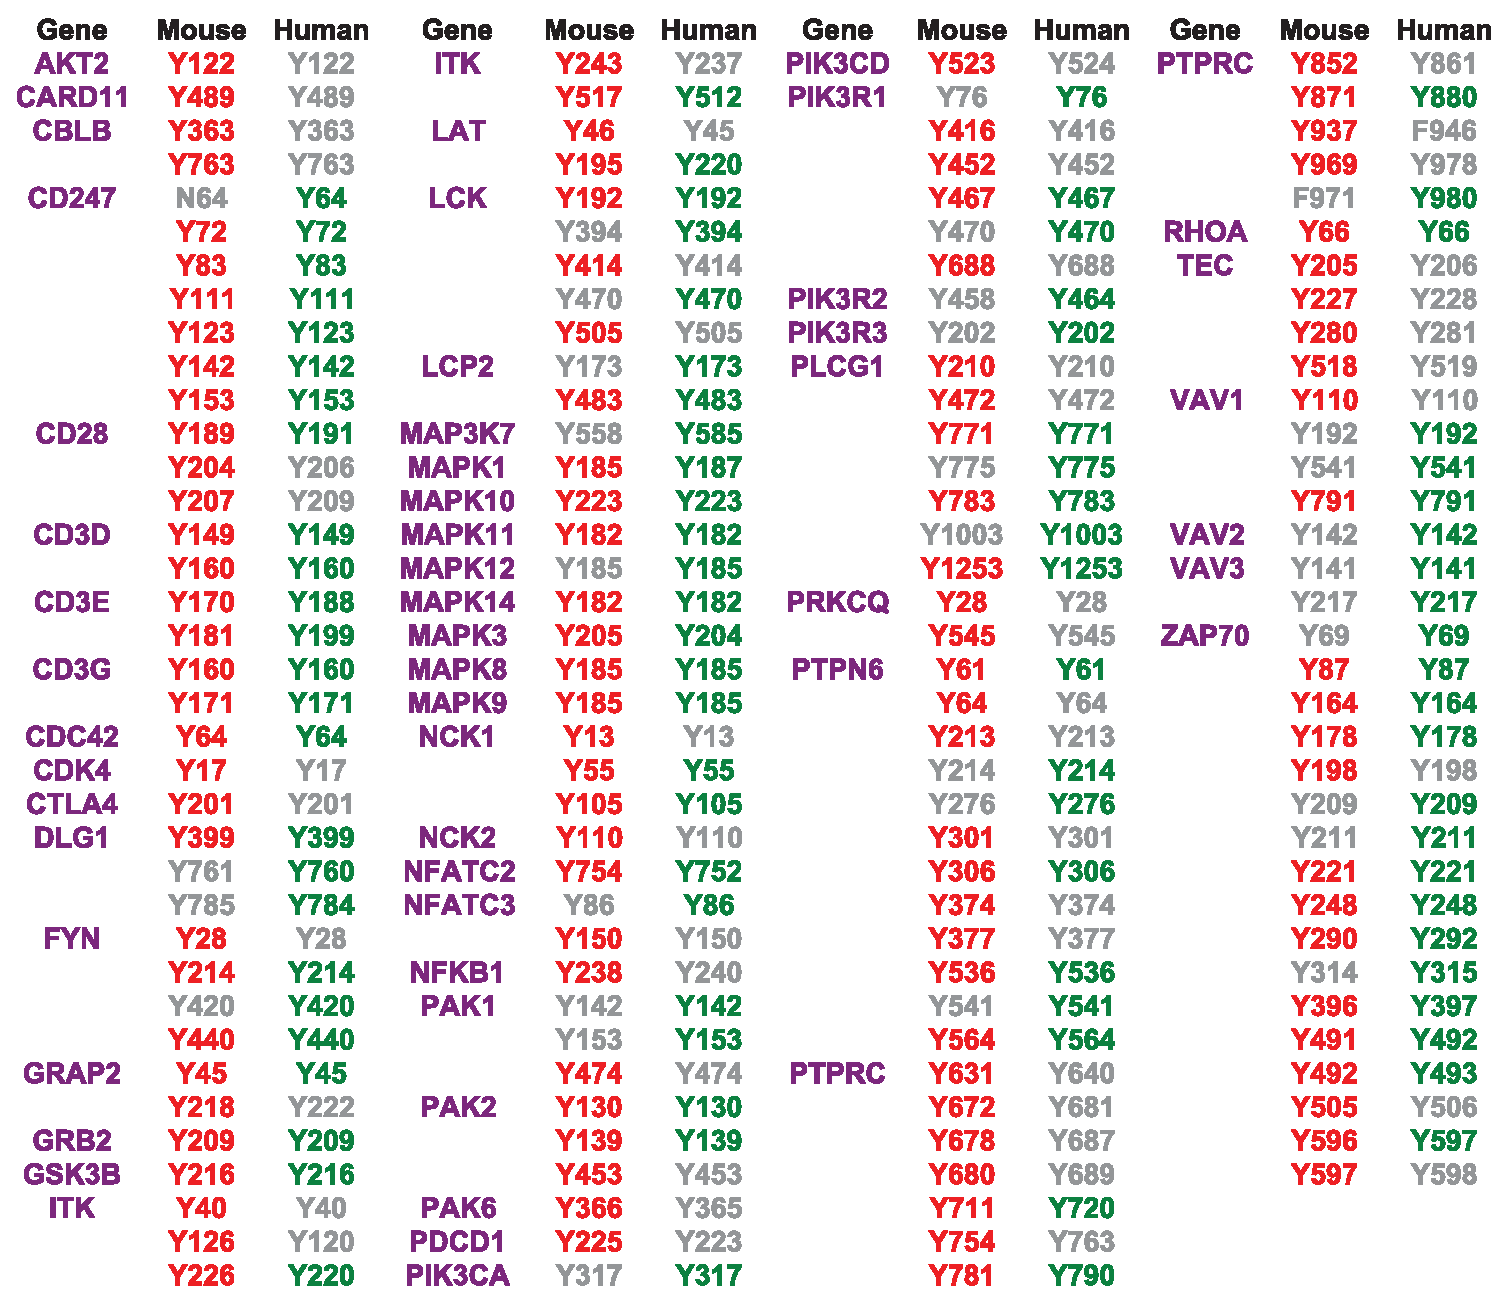
\includegraphics[width=165mm]{figures/supplements/mouse_jurkat_keggtcr.pdf}
\caption{Comparison of pTyr sites identified using BOOST in primary T cells from mice and pTyr sites identified using BOOST in Jukat T cells. Flanking sequences (phosphorylation site $\pm7$ amino acids) and phosphorylation sites for each protein in the Kyoto Encyclopedia of Genes and Genomes T cell receptor signaling pathway were manually curated from \href{https://www.phosphosite.org}{PhosphoSitePlus$^{\text{\textregistered}}$}\cite{hornbeck2015phosphositeplus} for humans and mice. Flanking sequences for each peptide in the Mouse-BOOST and Jurkat-BOOST datasets were compared with the manually curated KEGG TCR/PhosphoSitePlus flanking sequences and filtered for unique sites. Gene names are colored \textbf{{\color{Purple}purple}}. Phosphotyrosine sites identified in mice are colored \textbf{{\color{Red}red}}. Phosphotyrosine sites identified in Jurkat T cells are colored \textbf{{\color{ForestGreen}green}}. Sites that were not identified either mice or Jurkat T cells are colored \textbf{{\color{Gray}grey}}. PSMs that can be assigned to multiple proteins: $\bm{\XOR}$Cbl-B;Cbl $|$ $^{\textbf{\%}}$CDC42/RHOA $|$ $^{\textbf{\$}}$Fyn/Yes1 $|$ $^{\textbf{*}}$Fyn/Yes1/Src/Lck $|$ $^{\textbf{!}}$Fyn/Yes1/Src $|$ $^{\textbf{\&}}$GSK3$\beta$/GSK3$\alpha$ $|$ $^{\textbf{\#}}$Jnk1/Jnk3 $|$ $^{\textbf{+}}$PAK1/PAK2. }\label{mouse_jurkat_keggtcr}
\end{figure}

\clearpage

\bibliography{citations.bib}

\end{document}




























